\documentclass[reprint,amsmath,amssymb,aps,pra]{revtex4-2}
\usepackage{bm}
\usepackage{amsmath,amssymb,graphicx,stmaryrd,tabularx}
\usepackage{xcolor}
\usepackage{float}
\usepackage{physics}
\usepackage[colorlinks=true]{hyperref}
\usepackage{chngcntr}
\usepackage{mathtools}
\usepackage{algorithm}
%\usepackage{float}
\usepackage[floatrow]{trivfloat}
\usepackage{dblfloatfix}
%\setlength{\parskip}{0.2em}
\usepackage{parskip}
\usepackage{csquotes}
\MakeOuterQuote{"}

%%%%%%%%%% Start TeXmacs macros
\newcommand{\assign}{:=}
\newcommand{\backassign}{=:}
\newcommand{\mathe}{\mathrm{e}}
\newcommand{\mathi}{\mathrm{i}}
\newcommand{\tmcolor}[2]{{\color{#1}{#2}}}
\newcommand{\tmem}[1]{{\em #1\/}}
\newcommand{\tmbf}[1]{\ensuremath{\boldsymbol{#1}}}
\newcommand{\tmname}[1]{\textsc{#1}}
\newcommand{\tmop}[1]{\ensuremath{\operatorname{#1}}}
\newcommand{\tmrsup}[1]{\textsuperscript{#1}}
\newcommand{\tmscript}[1]{\text{\scriptsize{$#1$}}}
\newcommand{\tmstrong}[1]{\textbf{#1}}
\newcommand{\tmverbatim}[1]{{\ttfamily{#1}}}
%%%%%%%%%% End TeXmacs macros

\newcommand{\iwn}{\mathrm{i}\omega_n}
\DeclareMathOperator{\sgn}{sgn}
\newcommand{\e}{\mathrm{e}}

\usepackage{titlesec}
\titlespacing*{\section}{0pt}{0.8\baselineskip}{0.6\baselineskip}
\titlespacing*{\subsection}{0pt}{0.8\baselineskip}{0.6\baselineskip}
\titlespacing*{\subsubsection}{0pt}{\baselineskip}{0.6\baselineskip}

\begin{document}

\title{A LISA DMFT to study the Mott transition in the Hubbard model}

\author{Félix Faisant}
\author{Romain Fouilland}
\author{Charles Boudet}
\affiliation{"Modern Electronic Structures Methods" project report. Master 2 ICFP, ENS Paris}

\date{January 04, 2021}

\begin{abstract}
Physics of the single orbital Hubbard model at half-filling is explored by implementing a LISA DMFT approach on a Bethe lattice, using Iterated Perturbation Theory as the impurity solver. It enables us to characterize both its metallic and Mott insulator phases, recovering the phase transition that lies between, up till a reconstitution of the $(\beta, U)$ phase diagram. Therebeyond, the physics at stake can be well understood by examining the spectral function $A(\omega)$, whose computation requires the solution of an analytical continuation problem. It is untangled through a machine learning approach which compares to, and may even outperform previous methods such as techniques based on Padé approximants. The formalism underpinning LISA DMFT and its numerical implementation is briefly exposed.
\end{abstract}

\maketitle

%\tableofcontents

At first sight, the description of metals by condensed matter theory looks paradoxical. Charge carriers are electrons, which are charged particles. Even if interactions are screened, we do not expect a free electron gas model to describe metals. Yet, most materials can be satisfyingly described by effectively non-interacting electrons models. Indeed, we often observe clean band structures using ARPES, and DFT predict them well... up to a certain amount of electron mass and energy renormalization. However, some materials (often insulating ones) fails to display band structure.

It is now understood that most metals are described well by Fermi liquid theory, where \emph{dressed} electrons behave as independent quasi-particles with renormalized properties, despite interactions. On the other hand, this picture fails in \emph{strongly correlated materials}. Some materials exhibit a transition between these two regimes, turning a metal into an \emph{Mott insulator}.

The \textbf{Hubbard model} is the simplest lattice model showing this Mott transition, the \emph{Drosophila} of condensed matter. We investigate its different phases using a dynamical mean-field theory, LISA DMFT.

\section{DMFT formalism and theory}

\subsection{The Hubbard model}

The Hubbard model is the simplest model to describe the interplay between
local Coulomb interactions and the kinetic energy. In this model, electrons are moving on a lattice\footnote{For instance, each site of the lattice can depict an atomic core.} by tunneling, and pay Coulomb interaction cost if there is double occupancy on a site. In particular, the Hamiltonian of a single-orbital nearest-neighbor Hubbard model on a lattice $\{ i \}$ is :
\begin{equation}
  \tmbf{H} = \underbrace{- \sum_{\langle i, j \rangle, \sigma}
  {\color[HTML]{008080}t_{i j}}  (\tmbf{c}_{i \sigma}^{\dag}
  \tmbf{c}_{j \sigma} +\tmbf{c}_{j \sigma}^{\dag} \tmbf{c}_{i
  \sigma})}_{\text{\footnotesize hopping / hybridization}} + \underbrace{{\color[HTML]{BF4040}U}  \sum_i \tmbf{n}_{i
  \uparrow} \tmbf{n}_{i \downarrow}}_{\clap{\text{\footnotesize Coulomb repulsion}}} \label{Hubbard-model}
\end{equation}

In the following, quantities in {\color[HTML]{008080}green} denote non-interacting properties (that is tight-binding, $U=0$) and {\color[HTML]{BF4040}red} denotes interacting properties. The hopping amplitudes ${\color[HTML]{008080}t_{i j}}$ (and thus the model) are translationally invariant. The system will be considered in the grand canonical ensemble ($\tmbf{H}_{\mathrm{{\tmname{gc}}}} = \tmbf{H} - \mu \tmbf{N}$) at inverse temperature $\beta$ and half-filling, i.e. at a chemical potential $\mu$ such that $\langle \tmbf{n}_{i\uparrow} +\tmbf{n}_{i\downarrow} \rangle_{\mathrm{{\tmname{gc}}}} = 1$. Independently of $\beta$, we'll always have $\mu = {\color[HTML]{BF4040}U} / 2$.

The Hubbard model has been solved exactly in the one-dimensional and infinite-dimensional cases. The later case is where DMFT becomes exact \cite{Georges1996}. At zero temperature, two limits can be identified :

\paragraph{Non-interacting limit}

The $t \gg {\color[HTML]{BF4040}U}$ limit leads to full delocalization and
{\color[HTML]{008080}non-interacting} electrons, that is a tight-binding \emph{band} {\color[HTML]{008080}$\epsilon (\vec{k})$} and Bloch waves $\vec{k}$ :
\begin{equation}
  {\color[HTML]{008080}\tmbf{H}} =
  \sum_{\vec{k}}
  {\color[HTML]{008080}\epsilon (\vec{k})} \tmbf{c}_{\vec{k}}^{\dag} \tmbf{c}_{\vec{k}}
  \ \text{ with } \
  {\color[HTML]{008080}\epsilon (\vec{k})}  =  \sum_j -
  {\color[HTML]{008080}t_{i j}} \mathe^{\mathi \vec{k} \cdot \vec{R}_{i j}}
  \label{hubbard-non-interacting-band}
\end{equation}
The eigenstates of this hamiltonian are Slater determinants of Bloch waves, and the spectral function is then
\begin{equation}
  {\color[HTML]{008080}A_0} (\vec{k}, \omega) = \delta (\omega + \mu -
  {\color[HTML]{008080}\epsilon} (\vec{k})) \label{spectral-func-NIEG}
\end{equation}
at any temperature. Electrons can flow, and the system is metallic.

\paragraph{Atomic limit}

The ${\color[HTML]{BF4040}U} \gg t$ limit leads to a sum of isolated sites
$\smash{\tmbf{H}_{\mathrm{{\tmname{gc}}}}^{(1)} = {\color[HTML]{BF4040}U}
\tmbf{n}_{\uparrow} \tmbf{n}_{\downarrow} - \mu
(\tmbf{n}_{\uparrow} +\tmbf{n}_{\downarrow})}$. Electrons are localized on sites to minimize Coulomb interactions and can't flow. We thus have an insulator. The eigenstates are Slater determinants of localized states. The spectral function is then (at any temperature)
\begin{equation}
\label{atomic-limit-spectral-func}
 {\color[HTML]{BF4040}A} (\omega) = \tfrac{1}{2}\, \delta \left(
   \omega - \tfrac{{\color[HTML]{BF4040}U}}{2} \right) + \tfrac{1}{2}\, \delta
   \left( \omega + \tfrac{{\color[HTML]{BF4040}U}}{2} \right)
\end{equation}

\paragraph{Intermediate regime}

In between, there is a competition between delocalization and repulsion. A transition between the metallic and insulating phases happens. To investigate this regime computationally, we need to introduce the Green's function formalism.

\subsection{Green's function formalism}
\label{section:green_functions}

As it is impossible to compute directly the many-body wavefunction of the system since it lives in $\mathbb{R}^{10^{23}}$, we restrict ourselves to a formalism related to experimentally measurable quantities. In particular, the {\tmem{one-body spectral function}} $A (\vec{k}, \omega)$, or spectral density, is what is observed in one-electron removal (that is {\tmname{arpes}} experiments) and addition. It is related to the
{\tmem{one-body Green's function}}, which characterizes the fate of an electron injected into the system.

\subsubsection{Green's function in real and Matsubara time\label{sec:green-func}}

The \tmem{zero-temperature time-ordered one-body Green's function} is defined by
\begin{equation}
    G(i, t, j, t') = - \mathi \left\langle \mathrm{{\tmname{gs}}} \right|
    \tmbf{T}\tmbf{c}_i (t) \tmbf{c}_j^{\dag} (t')  \left|
    \mathrm{{\tmname{gs}}} \right\rangle
\end{equation}
in lattice position basis, where $\tmbf{T}$ is the time-ordering operator and $\left| \mathrm{{\tmname{gs}}} \right\rangle$ is the ground state. $\tmbf{c}(t)$ denote the operator in Heisenberg picture. Our problem is time-independent ($t'=0$) and $G$ depends only on $\vec{R}_{i j}$. Its spatial Fourier transform is denoted $\smash{G(\vec{k}, t)}$, and is linked to the spectral function by Fourier transform \footnote{\begin{equation}
    G (\vec{k}, \omega) = \int_{- \infty}^{+ \infty} \dd{\omega'} \frac{A(\vec{k}, \omega')}{\omega - \omega' + \mathi 0^+ \tmop{sgn} \omega'}
\label{green-func-from-spectral-func}
\end{equation}}.

At finite temperatures ($\beta < \infty$), working with real-time Green's functions is impractical and limited to real-time impurity solvers, which are involved and not used here. We rather switch to Matsubara time $\tau$ (or "imaginary" time). Then, the Heisenberg picture evolution is replaced by $\tmbf{c} (\tau) =
  \mathe^{\tmbf{H}_{\mathrm{{\tmname{gc}}}} \tau} \tmbf{c} \mathe^{-\tmbf{H}_{\mathrm{{\tmname{gc}}}}
  \tau}$, and we define the Matsubara Green's function (which is real)
\begin{equation}
    G_{\beta} (i,j,\tau) = \tfrac{1}{Z} \tr( \mathe^{- \beta \tmbf{H}_{\mathrm{{\tmname{gc}}}}}
    \tmbf{T}\tmbf{c}_i (\tau) \tmbf{c}_j^{\dag} (0))
\label{matsubara-green-func-def}
\end{equation}

It is \tmem{anti-periodic} with period $\beta$ as $G (\tau) = - G (\tau + \beta)$ and can be restricted to $\tau \in [0,\beta]$. It is then decomposed as a Fourier series
\begin{equation}
    G_{\beta} (\tau) = \frac{1}{\beta}  \sum_{n = - \infty}^{+ \infty} \mathe^{-
    \iwn \tau} G_{\beta} (\iwn)
  \label{green-func-matsubara-IFT}
\end{equation}
where $\omega_n = \frac{2 n + 1}{\beta} \pi$ are {\tmem{Matsubara frequencies}}.\\
$G (\tau)$ being real, $G (\iwn)^{\ast} =
G_{\beta} (- \iwn)$ and we only need to know $G(\iwn)$ for frequencies $n \in \llbracket 0, + \infty \llbracket$. The behavior at $\tau \rightarrow 0$ is singular : there is a discontinuity $G (\tau \rightarrow 0^+) - G (\tau \rightarrow 0^-) = - 1$. The Matsubara Green's function $G_{\beta} (\iwn)$ is simply the analytic continuation of the retarded Green's function, evaluated on the imaginary axis $t = -\mathi \tau \Leftrightarrow \iwn = \omega + \mathi 0^+$. Similar to (\ref{green-func-from-spectral-func}), it is connected to the spectral function :
\begin{equation}
    G_{\beta} (\vec{k}, \iwn) = \int_{- \infty}^{+ \infty} \dd{\omega'} \frac{A (\vec{k}, \omega')}{\iwn - \omega'}\\
\label{green-func-matsubara-freq-from-spectral-func}
\end{equation}
which has to be inverted to get back $A (\vec{k}, \omega)$. However, this is unfortunately an ill-defined problem and we'll have to resort to approximate inversion methods.

For the non-interacting electron gas, the Matsubara Green's
function is, using (\ref{spectral-func-NIEG}) and (\ref{green-func-matsubara-freq-from-spectral-func}), \footnote{
In Matsubara time space, we have ${\color[HTML]{008080}G_{0, \beta}} (\vec{k}, \tau) = -
   \mathe^{({\color[HTML]{008080}\epsilon} (\vec{k}) - \mu)  (\beta - \tau)}
   f^{\mathrm{{\tmname{fd}}}}_{\beta} ({\color[HTML]{008080}\epsilon}
   (\vec{k}) - \mu)$ for $\tau \in] 0, \beta [$, and where  $f^{\mathrm{{\tmname{fd}}}}_{\beta} (\epsilon)$ is the Fermi-Dirac distribution.
}
\begin{equation}
  {\color[HTML]{008080}G_{0, \beta}} (\vec{k}, \iwn) =
  \frac{1}{\iwn - {\color[HTML]{008080}\epsilon} (\vec{k}) + \mu}
  \label{green-func-matsubara-non-interacting}
\end{equation}

If we have particle-hole symmetry (which is the case at half-filling; abbreviated "p-h"), then $A (-\omega) = A (+\omega)$. As a consequence, $G (\iwn)^{\ast} = {- G (\iwn)}$, so that \emph{it has no real part}. This condition is important in practice.

\subsubsection{Local part of the Green's function}

More specifically, an central quantity in DMFT is the \emph{local Green's function}
$G_{\text{loc}} \assign G_{i i}$ (i.e.~$\vec{R} = \vec{0}$), which describes
the process "an electron stays on the site". The
{\color[HTML]{008080}non-interacting} local Green's function in Matsubara frequency space takes the simple form
\begin{equation}
  {\color[HTML]{008080}G}_{{\color[HTML]{008080}0}, \text{loc}} (\iwn) = {\color[HTML]{008080}\tilde{\eta}}\,(\zeta = \iwn + \mu) \label{G0loc-with-Hilbert-tr-DOS}
\end{equation}
where $\tilde{\eta}$ is the Hilbert transform $ {\color[HTML]{008080}\tilde{\eta}} (\zeta) = \int \dd{\epsilon} \frac{{\color[HTML]{008080}\eta} (\epsilon)}{\zeta - \epsilon} \label{Hilbert-tr-DOS} $ of the density of states ${\color[HTML]{008080}\eta}(\epsilon)$ of the lattice, computed from ${\color[HTML]{008080}\epsilon} (\vec{k})$.

\subsubsection{Self-energy}

A quantity easier to handle than Green's functions is the {\tmem{self-energy}}, which is the difference of the inverses of the interacting ${\color[HTML]{BF4040}G}$ and non-interacting ${\color[HTML]{008080}G_0}$ Green's functions :
\begin{equation}
  {\color[HTML]{BF4040}\Sigma} (\vec{k}, \iwn) = {\color[HTML]{008080}G_0}
  (\vec{k}, \iwn)^{- 1} - {\color[HTML]{BF4040}G} (\vec{k}, \mathi
  \omega_n)^{- 1}
\end{equation}
This is the \emph{Dyson equation}. The self-energy encodes all one-body interactions properties : Hartree energy, exchange and correlations.

Because the non-interacting problem has a known solution in term of a band $\smash{{\color[HTML]{008080}\epsilon} (\vec{k})}$,
${\color[HTML]{008080}G_0}$ is known
(\ref{green-func-matsubara-non-interacting}). Then, the interacting Green's function can be written
\begin{equation}
    {\color[HTML]{BF4040}G} (\vec{k}, \iwn) = \frac{1}{\iwn -
    {\color[HTML]{008080}\epsilon (\vec{k})} + \mu -
    {\color[HTML]{BF4040}\Sigma} (\vec{k}, \iwn)}\\
\label{interacting-green-func-self-energy}
\end{equation}
It implies that the interactions, via the self-energy
${\color[HTML]{BF4040}\Sigma}$, {\tmem{modifies the poles}} (in a temperature-dependant way). And because ${\color[HTML]{BF4040}\Sigma}\in \mathbb{C}$, it gives \emph{finite lifetime} to the excitations (i.e.\ adds width to the bands in the spectral function), and renormalizes their masses and energies. 

From (\ref{interacting-green-func-self-energy}), the local Green's
function ${\color[HTML]{BF4040}G}_{\text{loc}} (\iwn) =
{\color[HTML]{BF4040}G}_{i i} (\iwn) = \smash{\sum_{\vec{k}}{\color[HTML]{BF4040}G} (\vec{k}, \iwn)}$ can be
expressed with density of states of the non-interacting
problem, as for (\ref{G0loc-with-Hilbert-tr-DOS}) :
\begin{equation}
    {\color[HTML]{BF4040}G}_{\text{loc}} (\iwn) =
    {\color[HTML]{008080}\tilde{\eta}}\, \big({\color[HTML]{BF4040}\zeta} = \mathi
    \omega_n + \mu - {\color[HTML]{BF4040}\Sigma}_{\text{loc}} (\iwn)\big)
\label{Gloc-with-Hilbert-tr-DOS}
\end{equation}

\subsection{Dynamical Mean-Field Theory}

\subsubsection{The mean-field approximation}

In infinite dimensions, each site has an infinite number of neighbors. Therefore, by the law of large numbers, \emph{correlations between sites vanish} and \emph{quantum fluctuations become purely local}. Then, every electron is bathed in a \emph{mean field} determined by immediate neighbors only. Still, quantum fluctuations occurs. It is thus a \emph{dynamical} mean-field theory. This is no more the case in finite dimensions, but we still use DMFT as an approximation. In the Green's function framework, the statement "fluctuations become purely local" means a \emph{purely local self-energy} :
\begin{equation}
    {\color[HTML]{BF4040}\Sigma}_{i j} 
    \overset{\text{{\tmname{dmft}}}}{\approx} 
    {\color[HTML]{BF4040}\Sigma}_{\text{loc}} \delta_{i j}\\
    \quad \Leftrightarrow \quad {\color[HTML]{BF4040}\Sigma}
  (\vec{k})  \approx {\color[HTML]{BF4040}\Sigma}_{\text{loc}}
  \label{DMFT-local-approx}
\end{equation}
where ${\color[HTML]{BF4040}\Sigma}_{\text{loc}}$ is a \emph{single} number (spatially-wise). \footnote{The Green's function (\ref{interacting-green-func-self-energy}) then becomes \begin{equation*}
{\color[HTML]{BF4040}G} (\vec{k}, \iwn) \approx \frac{1}{\iwn - {\color[HTML]{008080}\epsilon (\vec{k})} + \mu - {\color[HTML]{BF4040}\Sigma}_{\text{loc}} (\iwn)}\end{equation*}
which summarizes well the spirit of DMFT. But we don't need this expression as we'll only look at $G_\text{loc}$, that is $A(\omega)$, rather than the full $A(\vec{k},\omega)$.}

\subsubsection{An impurity model}

A mean-field theory needs two ingredients :
\begin{itemize}
    \item An \textbf{auxiliary system} that is useful and can be solved. Here, given the previous remarks, the lattice problem naturally maps onto an \textit{impurity model}, as illustrated on fig.\ \ref{fig:sch-impurity-mapping}.
    \item A \textbf{mean-field equation} to implement the symmetries of our original problem. Here, these are the translational invariance and the coherence effects of our lattice problem. It is performed using the cavity method\cite{Georges1996}.
\end{itemize}

\begin{figure}[H]
\centering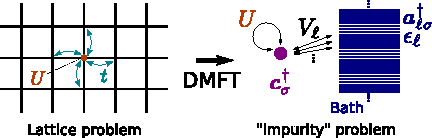
\includegraphics[width=\columnwidth]{mapping-impurity-compressed.pdf}
\caption{\label{fig:sch-impurity-mapping}Illustration of the mapping of the Hubbard model onto an impurity model, justified by the DMFT approximation. Double occupancy of the impurity $\tmbf{c}_{\sigma}^{\dag}$ is penalized, it exchanges electrons with a bath, which can be seen as an continuum of levels $\ell$.}
\end{figure}

The impurity model is described in sec.~\ref{impurity_model_section}. Suffice to say that it is a single fermion $\tmbf{c}_{\sigma}^{\dag}$ in interaction with a {\color[HTML]{000080}bath}, and with double-occupancy penalized by Coulomb interaction ${\color[HTML]{BF4040}U}$. We'll drop ${\sigma}$ in the following as our system will \emph{not be spin-polarized}. Its Green's function is
\begin{equation}
  {\color[HTML]{BF4040}G}^{\text{imp}}(t) = -\mathi \langle \tmbf{T} \tmbf{c}(t)  \tmbf{c}^{\dag}(0) \rangle
  \label{Gimp-def}
\end{equation}
and we consider as before its extension in Matsubara space ${\color[HTML]{BF4040}G}^{\text{imp}}(\iwn)$, as well as its self-energy ${\color[HTML]{BF4040}\Sigma}^{\text{imp}}(\iwn)$. The central equation is the \emph{self-consistency condition}
\begin{equation}
    \text{local Hubbard $\rightarrow$\quad}
    {\color[HTML]{BF4040}G}_{\text{loc}}^{\text{latt}} \overset{!}{=}
    {\color[HTML]{BF4040}G}^{\text{imp}}
    \quad \text{$\leftarrow$ impurity}
  \label{LISA-self-consistency}
\end{equation}
which imposes that the local part of the Green's function is identical to the impurity Green's function. This is the \textbf{LISA} (Local Impurity Self-consistent Approximation), where all spatial fluctuations are neglected. Finally, the bath (i.e.\ the mean-field) is described by a Green's function ${\color[HTML]{000080}\mathcal{G}_0}(\tau)$, and is determined by the mean-field equation
\begin{equation}
    \frac{1}{{\color[HTML]{000080}\mathcal{G}_0}(\iwn)} = {\color[HTML]{BF4040}\Sigma}_\text{loc}(\iwn) + \frac{1}{{\color[HTML]{BF4040}G}_\text{loc}(\iwn)}
    \label{mean_field_equation}
\end{equation}
in which we inject the relation between ${\color[HTML]{BF4040}\Sigma}_\text{loc}(\iwn)$ and ${\color[HTML]{BF4040}G}_\text{loc}(\iwn)$ imposed by the lattice, such as (\ref{Gloc-with-Hilbert-tr-DOS}).

\subsubsection{The DMFT self-consistent loop}

The final ingredient is a \textbf{solver} for the impurity model, giving us ${\color[HTML]{BF4040}G}^{\text{imp}}$ as a function of
the bath ${\color[HTML]{000080}\mathcal{G}_0}$ and ${\color[HTML]{BF4040}U}$. With the self-consistency condition and the mean-field equation, we have a closed system of equation which we solve in an iterative manner self-consistently :

\begin{algorithm}[H]
\begin{itemize}
\setlength\itemsep{0em}
    \item[] $\mathcal{G}_0^{(0)} \gets \text{initial guess for }\mathcal{G}_0$
    \item[] \textbf{while} $\| G^{(m)} - G^{\left( m-1 \right)} \| <
\varepsilon_{\text{thresh}}$:
    \item[] \hspace{2em} $G^{(m)}$ \hspace{0.4em} $\gets \operatorname{Impurity-Solver}[\mathcal{G}_0^{(m)}, {\color[HTML]{BF4040}U}]$ \textcolor{gray}{\ \# \textit{see eq.~\eqref{IPT}}}
    \item[] \hspace{2em} $G_{\text{loc}}^{\text{latt}}$ \hspace{0.5em} $\gets G^{(m)}$ \textcolor{gray}{\ \# \textit{see eq.~\eqref{LISA-self-consistency}}}
    \item[] \hspace{2em} $\mathcal{G}_0^{(m + 1)} \gets  \operatorname{Mean-Field}[G_{\text{loc}}^{\text{latt}}]$ \textcolor{gray}{\ \# \textit{see eq.~\eqref{self-consistent-eq-reciproc-Hilbert}}}
    \item[] \hspace{2em} \textbf{incr} $m$
    \item[] \textbf{yield} $G^{(m)}$
\end{itemize}
\caption{DMFT loop}\label{DMFT-loop}
\end{algorithm}

The DMFT loop can alternatively be written in terms of $\Sigma_\text{loc}(\iwn)$ depending on the mean-field equation used :
\begin{itemize}\setlength\itemsep{0em}
    \item $G_\text{loc}$-based with \eqref{self-consistent-eq-reciproc-Hilbert}
    \item $\Sigma_\text{loc}$-based with \eqref{mean_field_equation} and \eqref{Gloc-with-Hilbert-tr-DOS}; this is preferable for lattices with no analytical density of states ${\color[HTML]{008080}\eta}(\epsilon)$ available.
\end{itemize}

\subsection{Iterated Perturbation Theory}

The iterated perturbation theory (IPT) is a second order perturbation
theory in ${\color[HTML]{BF4040}U}$, solving the impurity problem. The self-energy is approximated by
\begin{equation}
    {\color[HTML]{BF4040}\Sigma}^\text{imp} (\iwn) \simeq \frac{{\color[HTML]{BF4040}U}}{2} + {\color[HTML]{BF4040}U}^2 
    \int_0^{\beta} \dd{\tau} \mathe^{\iwn \tau} 
    {\color[HTML]{000080}\mathcal{G}_0'} (\tau)^3
\label{IPT} 
\end{equation}
where $ \frac{1}{{\color[HTML]{000080}\mathcal{G}_0'} (\iwn)} = \frac{1}{{\color[HTML]{000080}\mathcal{G}_0} (\iwn)} - \frac{{\color[HTML]{BF4040}U}}{2}$ \footnote{The shift ${\color[HTML]{000080}\mathcal{G}_0'}^{- 1} =
{\color[HTML]{000080}\mathcal{G}_0}^{- 1} - U / 2$ effectively removes the
Hartee part of the self-energy, and makes
${\color[HTML]{000080}\mathcal{G}_0'}$ particle-hole symmetric (i.e.
$\mathfrak{R}\mathfrak{e} {\color[HTML]{000080}\mathcal{G}_0'} (\mathi
\omega_n) = 0$).}. It turns out this approximation is not only exact in the non-interacting limit but \emph{also in the atomic limit}, though \emph{only at half-filling} \cite{Georges1996}. Hence, we hope that it captures (at least qualitatively) the intermediate-${\color[HTML]{BF4040}U}$ physics.

\subsection{The Fermi liquid phase}

The low temperature metallic phase is described by Fermi liquid theory, where long-lived quasi-particles exist. An important quantity is the \emph{quasi-particle weight} $0 < \mathcal{Z}_{\vec{k}} \leq 1$. In a Fermi liquid \-- where the spectral function can be represented as the addition of an incoherent background to a quasi-particle peak \-- $\mathcal{Z}_{\vec{k}}$ is the spectral weight of the peak, and is linked to the inverse quasi-particle lifetime. In particular, taking $z=\iwn$, if the self-energy is continuous or can be analytically continued near $z=0$, then we can express it as follows in Matsubara space :
\[
\Sigma(\vec{k}, z) = \Sigma(\vec{k}, z = 0) + z \pdv{\Sigma(\vec{k}, z)}{z}\bigg|_{z=0} + \mathcal{O}(z^2)
\]
If we actually are in a Fermi liquid phase,  $\pdv{\Sigma(\vec{k}, z)}{z}\big|_{z=0} \geq 0$ and the weight reads :
\begin{equation}
\mathcal{Z}_{\textbf{k}}^{-1} = 1 - \pdv{\Sigma(\vec{k}, z)}{z}\bigg|_{z=0}
\label{quasi-p-weight}
\end{equation}

\subsection{Bethe Lattice}

The Bethe lattice represents a lattice in hyperbolic geometry. It is widely used as a \emph{Drosophila} in DMFT. When the coordination number is infinite, its density of states is semi-circular and particle-hole symmetric :
\begin{equation}
    {\color[HTML]{008080}\eta_{\text{Bethe}}} (\epsilon)  = \tfrac{1}{2 \pi t^2}  \sqrt{4 t^2 - \epsilon^2} \quad \text{for} \quad | \epsilon | < 2 t 
\end{equation}
As it is an analytical function, along with its Hilbert transform ${\color[HTML]{008080}\widetilde{\eta_{\text{Bethe}}}} (\zeta)$, it simplifies the implementation. In the following, $t=1$ is fixed as the energy unit (band width of $4$). Because $A(\omega=0)=\eta(0)$ in the Fermi liquid phase, a metallic peak will always have an amplitude $1/\pi$.

Other lattices are implemented easily, but not discussed here as the results do not qualitatively differ.

\section{Numerical implementation}

The aforementioned DMFT loop is implemented in several ways, and a basic ($T,U$) phase diagram is computed. However, many interesting quantities need the spectral function $A(\omega)$, and reconstructing it from the Green's function is a challenge.

\subsection{The DMFT loop with IPT}

\begin{figure}[H]
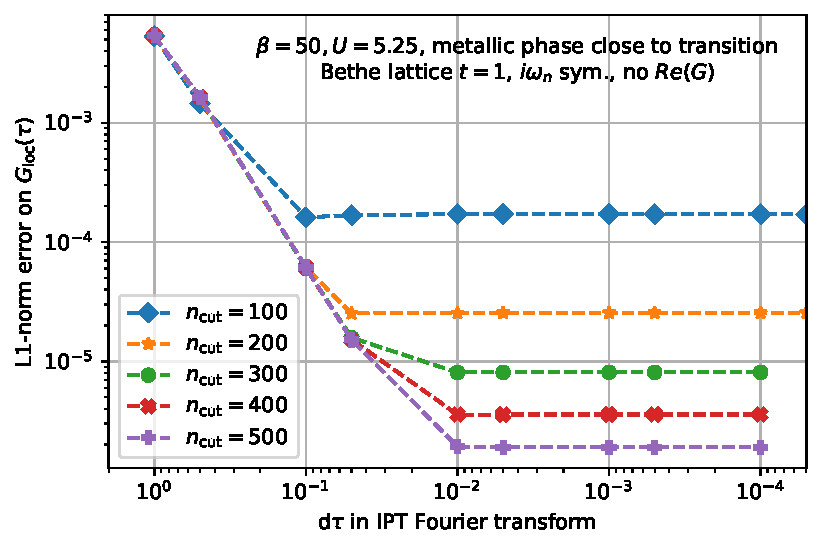
\includegraphics[width=\columnwidth]{Gloc-vs-Glocref.pdf}
\caption{\label{fig:conv-dtau-ncut}Error committed on the Green's function $G_\text{loc}(\tau)$ ($L^1$ norm in $\tau$ space) for varying $n_\text{cut}$ and $\dd{\tau}$, compared to a reference solution ($n_\text{cut}=600$, $\dd{\tau}=10^{-4}$). The chosen $(\beta,U)$ is close to the phase transition, and thus very sensitive to numerical errors.}
\end{figure}

While the implementation of the DMFT loop is straightforward \footnote{Our python implementation is available at the address \url{https://github.com/romainfd/DMFT_solver/blob/main/dmft-phase-diagram.ipynb}}, several practicalities must be considered :
\begin{itemize}
    \item The Green's function in Matsubara time $G(\tau)$ displays a discontinuity of amplitude $1$ at $\tau=0$. In Fourier space, this corresponds to a slow decay $G(\iwn)\simeq 1/\iwn$ of high frequencies. As infinitely many frequencies can't be considered on a computed, a cutoff $n<n_\text{cut}$ introduces Gibbs ringing when performing the inverse Fourier transform (iFT). To eliminate this problem, the iFT is performed after subtracting the $1/\iwn$ tail, and the corresponding term $\sgn \tau$ is added afterwards (a comparison is shown on fig.\ \ref{fig:green-tau-compar-sing}) : \begin{equation} G (\tau) = \frac{1}{\beta}  \sum_{n} \left( G (\iwn) - \frac{1}{\iwn} \right) \e^{-\iwn\tau} - \frac{\sgn \tau}{2} \label{iFT-sing}\end{equation}
    
    \item For IPT, we have to compute the integral (\ref{IPT}) over $\tau \in [0,\beta]$. The choice of the discretization step $\dd{\tau}$ is important. A smaller step is better, but much more costly in computation time. To choose $\dd{\tau}$ and $n_\text{cut}$, we make them vary for given parameters, as shown on fig.\ \ref{fig:conv-dtau-ncut}. A larger $n_\text{cut}$ always improve bellow $1000$, but $n_\text{cut}=300$ is chosen as a compromise with computation time. Then, $\dd{\tau}=5\cdot 10^{-3}$ is chosen, as a smaller step would not improve precision.

    \item The initial guess in the DMFT loop plays the role of an initial condition. The Mott transition being a first-order phase transition (under a certain temperature $T_c$), there is \emph{meta-stability} when increasing or decreasing $U$. Thus, \emph{the initial guess matters}.
    
    \item Over much of the $(U,\beta)$ phase diagram, the IPT-based DMFT loop is stable and converges towards a p-h symmetric solution, as expected. However, at low temperatures and close the the phase transition, a naive loop is \emph{unstable}. A real part can develop on $G_\text{loc}(\iwn)$, so that the system is no longer p-h symmetric (see fig.\ \ref{fig:ph-diag-sanity-checks}.a). Most often, this real part eventually decays, but it can still change the width of the hysteresis cycle (i.e. change the position and size of the coexistence zone on the phase diagram). While this may have a physical relevance, we decide to \emph{enforce particle-hole symmetry} by canceling $\mathfrak{Re}(G_\text{loc}(\iwn))$. Moreover, the conjugation property on negative frequencies (sec.\ \ref{sec:green-func}) must be strictly enforced or numerical instabilities may develop. \footnote{See the accompanying animations of the DMFT loop : \url{DMFTloop-beta_200-increasingU_5.25-transition-final_Re_cancel.mp4} for a real-part-induced phase transition, and \url{DMFTloop-beta_50-increasingU_5.25-transition-nonsym-noRe.mp4} for numerical instabilities due to lack of frequency-symmetry.}
\end{itemize}

\subsection{Spectral function reconstruction}

The spectral function $A (\vec{k}, \omega)$ is a key quantity : it is experimentally measured in \tmname{arpes} experiments, and is necessary to compute most properties such as conductivity. It is related to the Matsubara Green's function by the integral equation (\ref{green-func-matsubara-freq-from-spectral-func}). Inverting this equation to obtain $A (\vec{k}, \omega)$ is an ill-posed problem and cannot be solved exactly. It can be seen as an \emph{analytic continuation of $G(\iwn)$ from imaginary time to real time $G(\omega)$}.

\subsubsection{Machine learning approach}
Machine learning techniques are often used to learn data representation through training and are therefore relevant to our reconstruction problem. These techniques have been used for both Neural Networks \cite{NN_article} and Convolutional Neural Networks \cite{CNN_article}, which have been trained and analysed for our problem.

The problem to address being the inversion of $f : A(\omega) \mapsto G(\iwn)$ (\ref{green-func-matsubara-freq-from-spectral-func}), this allows for the generation of as many training points $(A(\omega),f[A(\omega)])$ as desired. 100,000 spectral densities are randomly generated using Gaussian shape peaks and evenly distributed between typical metallic and insulator spectral densities. For each one, $G(\iwn)=f[A(\omega)]$ is evaluated. As we restrict ourselves to p-h symmetric solutions, only the imaginary part of the first $n_\text{cut}=300$ positive Matsubara frequencies are used as the input data features.

Using this data to supervise learning, Neural Networks and Convolutional Neural Networks are trained. Early results from these networks have been used to determine a few key parameters, and the determination of the remaining ones is discussed below.

\subsubsection{Networks structure}

\begin{itemize}
    \item \emph{Learning} is actually an optimization of the weights of the network in order to obtain the desired outputs. It is done by gradient descent using the Adam optimizer (see sec.~\ref{sec:nn:grad-desc} for details). The gradient descent is stopped after 20 steps as there is no improvements on the validation data past this point. Such \emph{early stopping} prevent over-fitting.
    \item ReLU were used as activation functions as they gave better results than sigmoid activation functions and were more stable than SeLU and eLU activation functions.
    \item Dropout layers \footnote{This means that at each step of gradient descent, half of the nodes (randomly chosen) are simply forgotten and not updated. This forces the network to use all of the input features and all of its neurons instead of relying on subsets of them.} were used to prevent over-fitting (particularly for the CNN). A rate of 0.5 was chosen as a compromise with learning speed.
\end{itemize}

\begin{figure}[H]
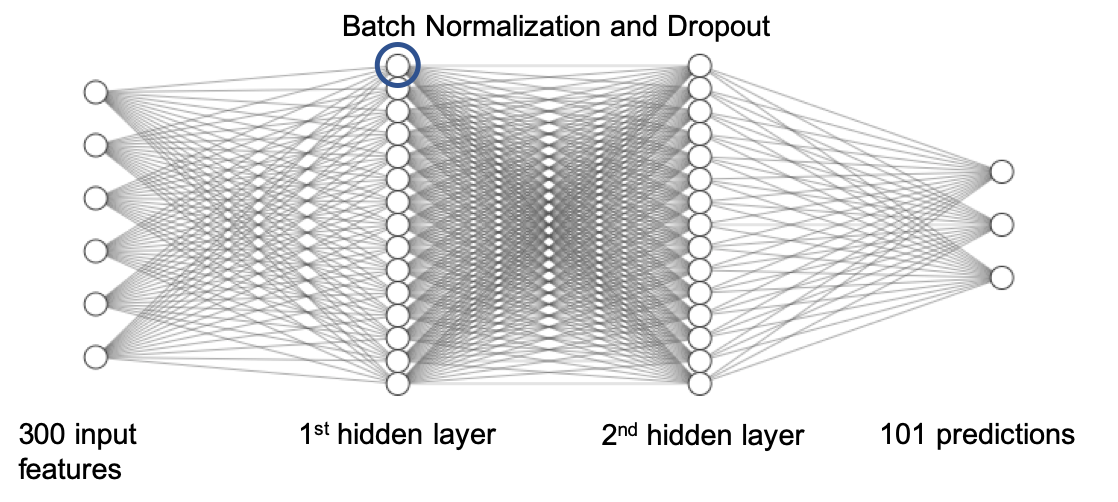
\includegraphics[width=\columnwidth]{analytical_continuation/NN_architecture.png}
\caption{\label{fig:NN_archi}Architecture of a Neural Network with 2 hidden layers.}
\end{figure}

\subsubsection{Loss function}

\begin{figure}[H]
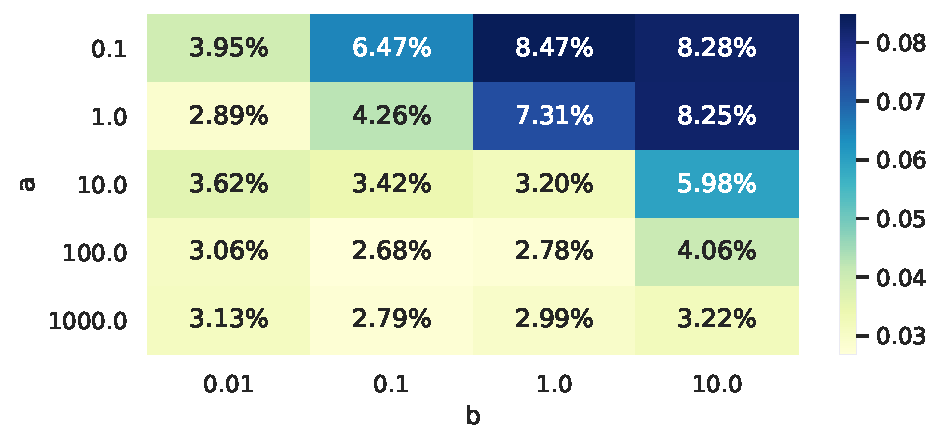
\includegraphics[width=\columnwidth]{analytical_continuation/norm_weighting_a_b2.pdf}
\caption{\label{fig:norm_a_b}Grid search on the weights of the values ($a$) and gradient ($b$) differences in the loss function to optimize the MAE.}
\end{figure}

Considering the training set, the loss function tells how close a predicted output $A_\text{pred}(\omega)$ is to the known exact solution $A_\text{true}(\omega)$.
Independently of the structures of the neural network, the use of $L^1$ and $L^2$ norms led to spectral densities matching well, but presenting a lot of noise and discontinuities. A key feature of machine learning approaches is to be "domain-knowledge" free. Encoding more features of the problem than those described above (frequency and p-h symmetry) would imply loosing this advantage. Still, changing the loss in order to promote continuity of the output $A(\omega)$ is not too specific. A loss function weighting the difference of value \emph{and} the gradient difference between $A=A_\text{pred}$ and $A_\text{true}$ is thus considered :
\begin{equation*}
    \ell(A, A_\text{true}) = a \| A - A_\text{true} \|_p + b \| \nabla_{\omega} A - \nabla_{\omega} A_\text{true} \|_p
\end{equation*}
where $\|\cdot\|_p$ is the $L^p$ norm and $a,b$ are weights to be optimized. To perform this parameter optimization and to compare results independently of the selected loss, the mean absolute error (MAE) was used. The $L^2$ norm performs better and was chosen (see sec~\ref{sec:nn:norm}). A grid search on $a$ and $b$ is performed. Figure~\ref{fig:norm_a_b} leads us to select the stable minimum $(a=100,b=0.1)$.

\subsubsection{Neural Networks}

\begin{figure}[H]
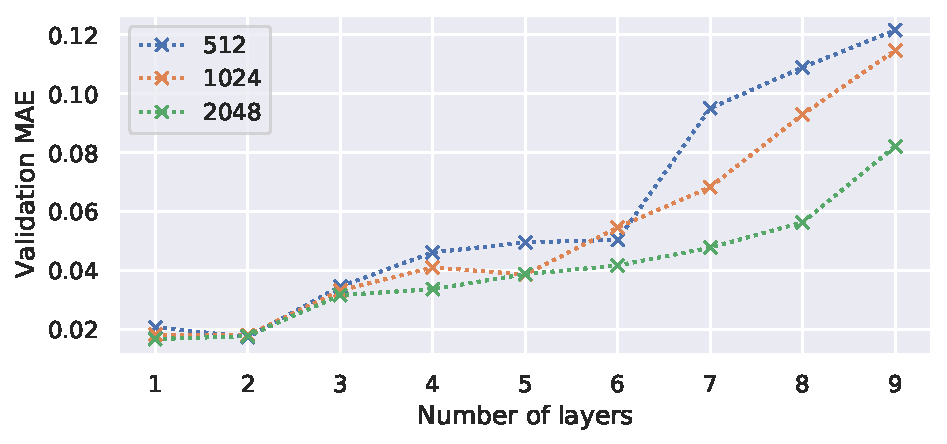
\includegraphics[width=\columnwidth]{analytical_continuation/NN_nb_layers.pdf}
\caption{\label{fig:NN_nb_layers}Evolution of the validation MAE for the Neural Network with the number of layers for number of neurons.}
\end{figure}

1. \emph{Number of layers.}\quad The first parameter to determine before further investigations of our Neural Network is the number of layers it should have. Figure~\ref{fig:NN_nb_layers} shows that one layer gives results with similar quality than 2 layers. For more layers, the network has too many parameters and starts over-fitting the training data. After a few iterations on the other parameters, it turned out one layer yields similar and even better results than two layers. As it is faster to train and should generalise better than deeper networks, we investigate a one hidden layer neural network.

2. \emph{Number of neurons.}\quad As weights and dropout layers introduce randomness in the trained models, 10 trainings are run for each number of neurons (similar approach taken in the other parameter fitting but the observed dispersion was way lower). From the analysis displayed in Figure~\ref{fig:NN_nb_nueurons}, one hidden layer of 4096 neurons seems to be the most robust and accurate model. As it is usually only 30\% slower than models with smaller layers but is still very fast (the duration of a training is of 3 minutes), this is our selected configuration.

\begin{figure}[H]
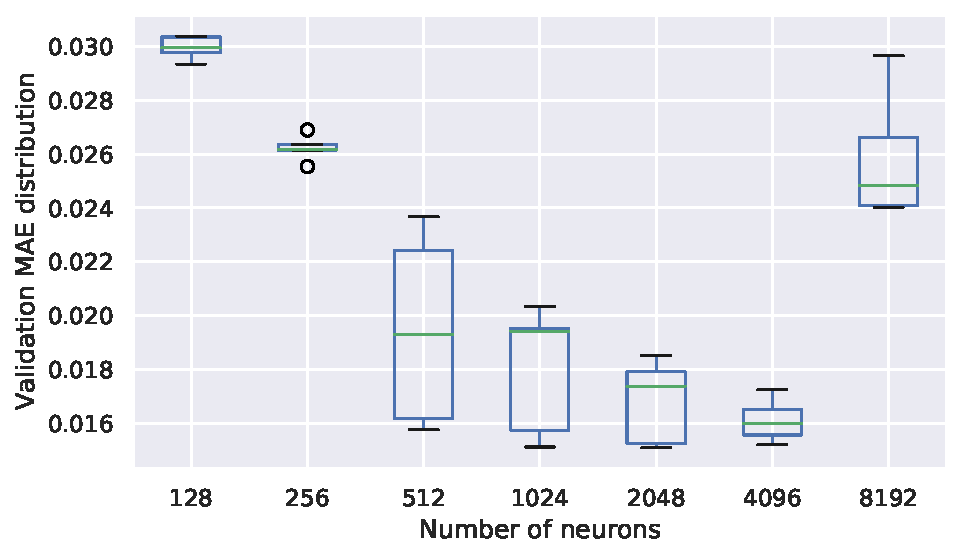
\includegraphics[width=\columnwidth]{analytical_continuation/NN_nb_neurons.pdf}
\caption{\label{fig:NN_nb_nueurons}Evolution of the validation MAE over time with different norms and weighting.}
\end{figure}

\subsubsection{Convolutional Neural Networks}
Neural Networks are good but don't take into account locality as they are dense layers connecting all the inputs to all neurons. To predict a function and to perhaps exploit results coming from the shape of the $G(\iwn)$ distribution, investigating Convolutional Neural Networks (CNNs) is relevant. The same parameter determination steps as for Neural Networks are reproduced for CNNs.

1. \emph{Number of layers.}\quad Different architectures have been tried by repeating a convolution layer of given size and adding a final dense layer before the output as illustrated in Figure~\ref{fig:CNN_archi}. For more convolutional layers, the Convolution and Max-Pooling layers would be repeated. Figure~\ref{fig:CNN_nb_layers} shows different architecture and indicates than one or two convolutional layers seems more promising.

\begin{figure}[H]
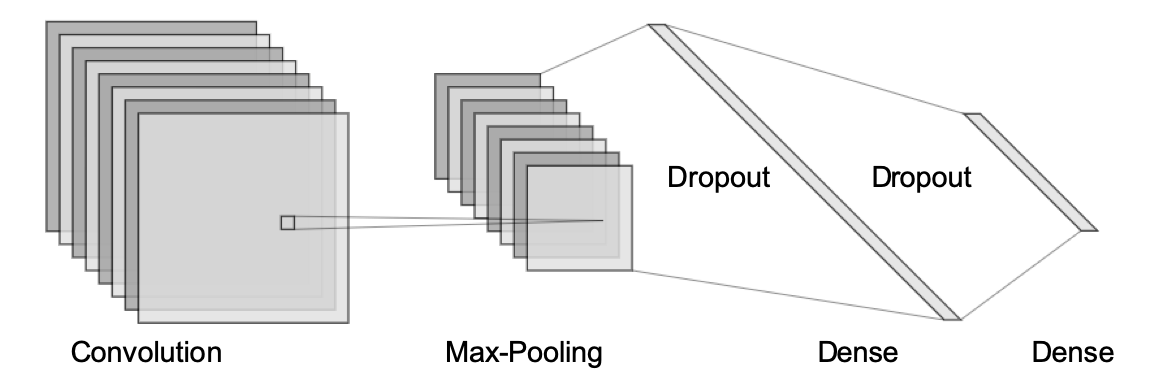
\includegraphics[width=\columnwidth]{analytical_continuation/CNN_architecture.png}
\caption{\label{fig:CNN_archi}Illustration of the CNN architecture for 3 layers (1 convolution and 2 dense ones). }
\end{figure}

\begin{figure}[H]
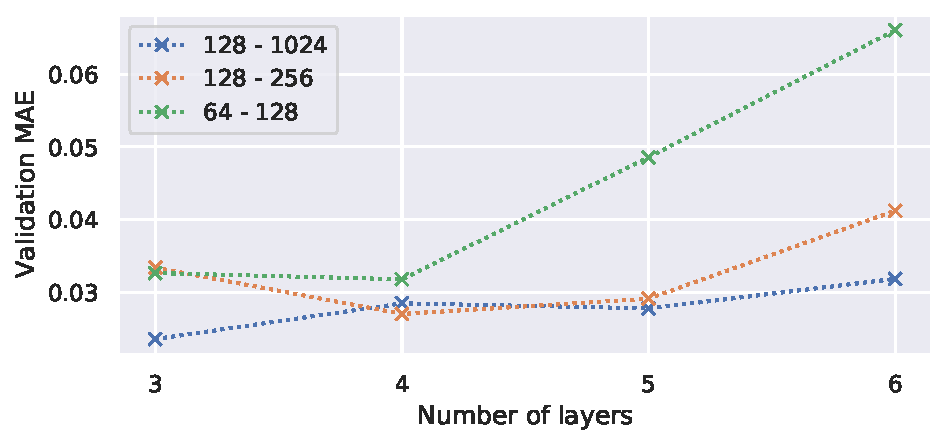
\includegraphics[width=\columnwidth]{analytical_continuation/CNN_nb_layers.pdf}
\caption{\label{fig:CNN_nb_layers}Evolution of the validation MAE for different number of layers. Architecture X-Y means the Convolutional layers use X kernels while the Dense layer before the output uses Y neurons.}
\end{figure}

2. \emph{Number of kernels.}\quad Convolutional layers use convolution kernels applied on the input. The same experiment as for the Neural Networks can be run for networks with one (fig~\ref{fig:CNN_nb_neurons_1layer}) and two convolutional layers (fig~\ref{fig:CNN_nb_neurons_2layer}). Best results are yielded for networks with only one convolutional layer using 256 kernels.
\begin{figure}[H]
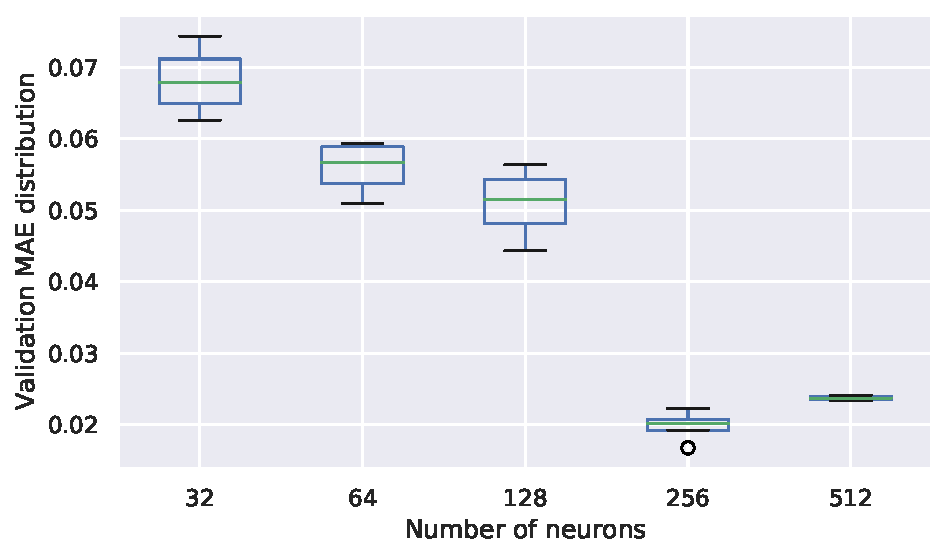
\includegraphics[width=\columnwidth]{analytical_continuation/CNN_nb_neurons.pdf}
\caption{\label{fig:CNN_nb_neurons_1layer}Evolution of the validation MAE with different number of kernels in a CNN with one convolution layer.}
\end{figure}
\begin{figure}[H]
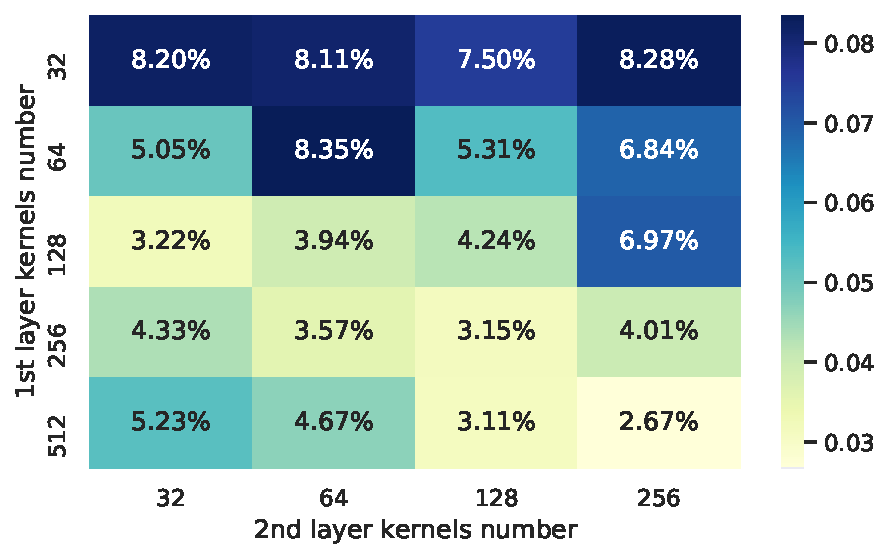
\includegraphics[width=\columnwidth]{analytical_continuation/CNN_nb_neurons_2layers2.pdf}
\caption{\label{fig:CNN_nb_neurons_2layer}Evolution of the validation MAE with different number of kernels in a CNN with two convolution layers.}
\end{figure}

\subsubsection{Padé comparison}

\begin{figure}[H]
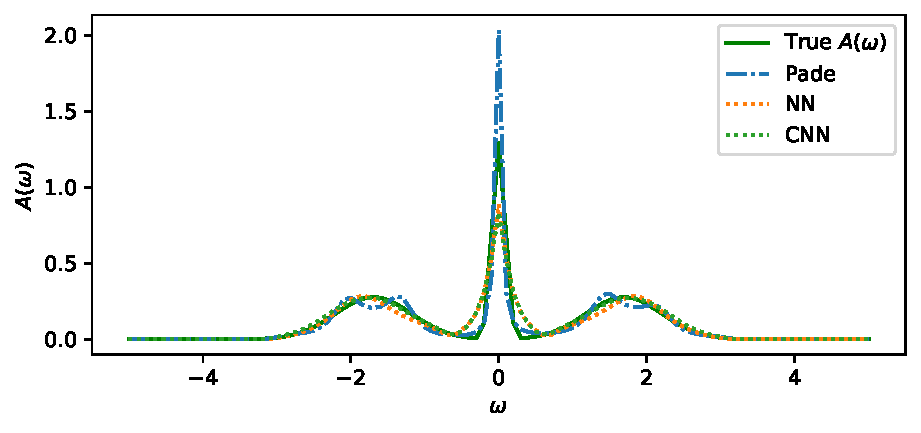
\includegraphics[width=\columnwidth]{analytical_continuation/pade_comp_metal.pdf}
\caption{\label{fig:compa_metal}Comparison of models with Padé reconstruction for metallic spectrum.}
\end{figure}
\begin{figure}[H]
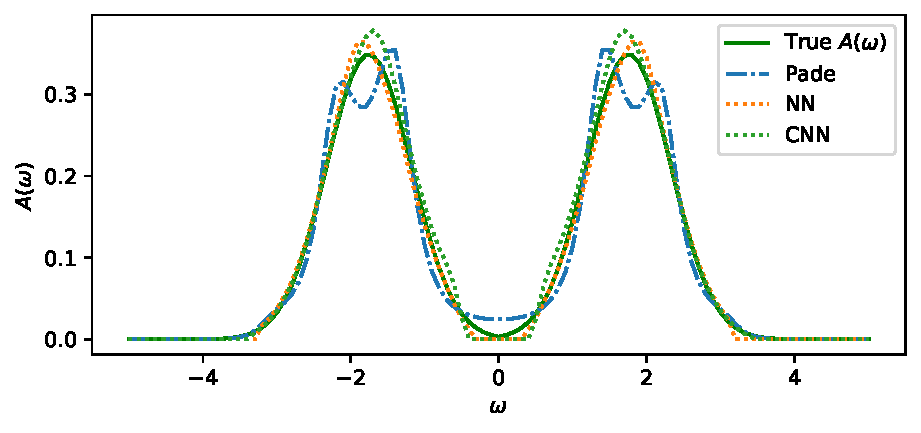
\includegraphics[width=\columnwidth]{analytical_continuation/pade_comp_isolant.pdf}
\caption{\label{fig:compa_isolant}Comparison of models with Padé reconstruction for insulator spectrum.}
\end{figure}

Using all the above parameter tuning, both an optimal Neural Network and Convolutional Neural Network have been determined with average MAE on the validation dataset of more than 30 thousands unseen density functions are 1.44\% for the Neural Network and 1.97\% for the Convolutional one. As before the norm optimization, even the best networks didn't reach an accuracy better than 5\%, these final accuracies seem highly satisfactory. However, to truly validate them, they should be compared to another analytic continuation solution and tested on real data.

To assess their accuracy level, we compare them with analytic continuation with Padé decomposition. As we can see on Figures~\ref{fig:compa_metal} and \ref{fig:compa_isolant}, our models and Padé behave well on both the insulator and metallic spectrums with similar performances.

Our models actually performed better on our generated spectrum densities. For new densities (not used for training or validation of the networks), our Neural and Convolutional Networks perform respectively 37\% and 11\% better (50\% for both if we look at the worst 10\%) as well as 200\% and 40\% faster than Padé reconstruction.

As seen on Figure~\ref{fig:compa_isolant}, Padé reconstruction seems a bit less continuous and struggling to reconstruct the very sharp peak of the metallic spectrum. These difficulties could be caused by the Gaussian shape of the generated spectrums and bias the results towards our models. Using our models and Padé reconstruction on the outputs of the DMFT solver presented above is interesting to dive deeper in the capabilities of the different analytic continuation tools.
 
\section{Results}

\begin{figure}[H]
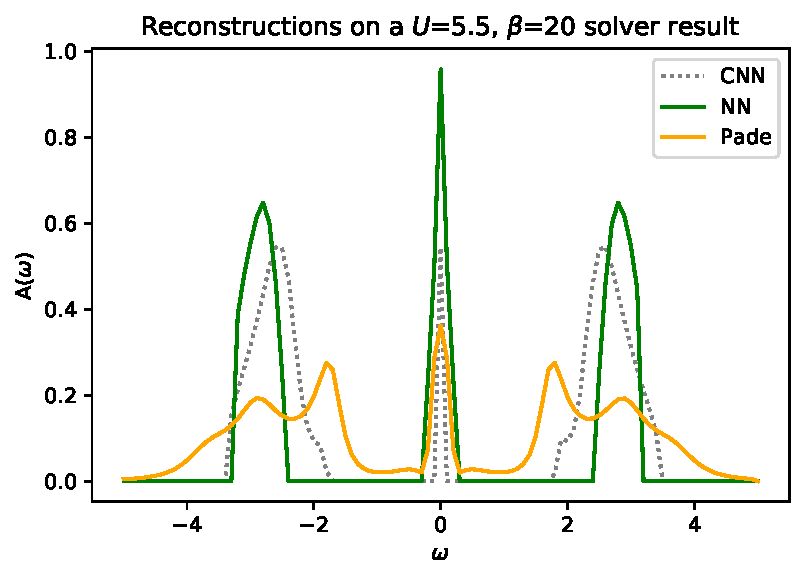
\includegraphics[width=0.9\columnwidth]{pred-metal.pdf}
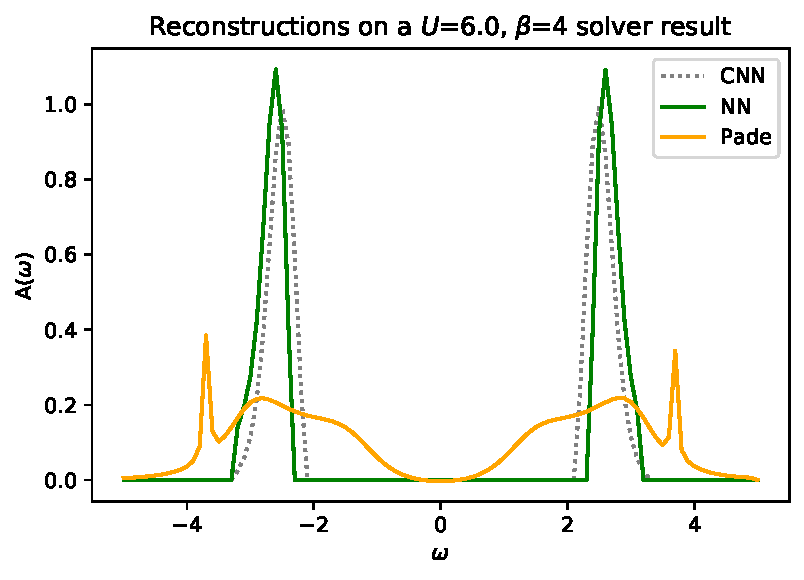
\includegraphics[width=0.9\columnwidth]{pred_isolant.pdf}
\caption{\label{fig:reconstr-final}Reconstructions of $A(\omega)$ with the trained CNN and NN, against the reconstruction with Padé approximants. Top: a metallic state near the tri-critical point. Bottom: an insulating state at high temperature.}
\end{figure}

\onecolumngrid

\begin{figure}[H]
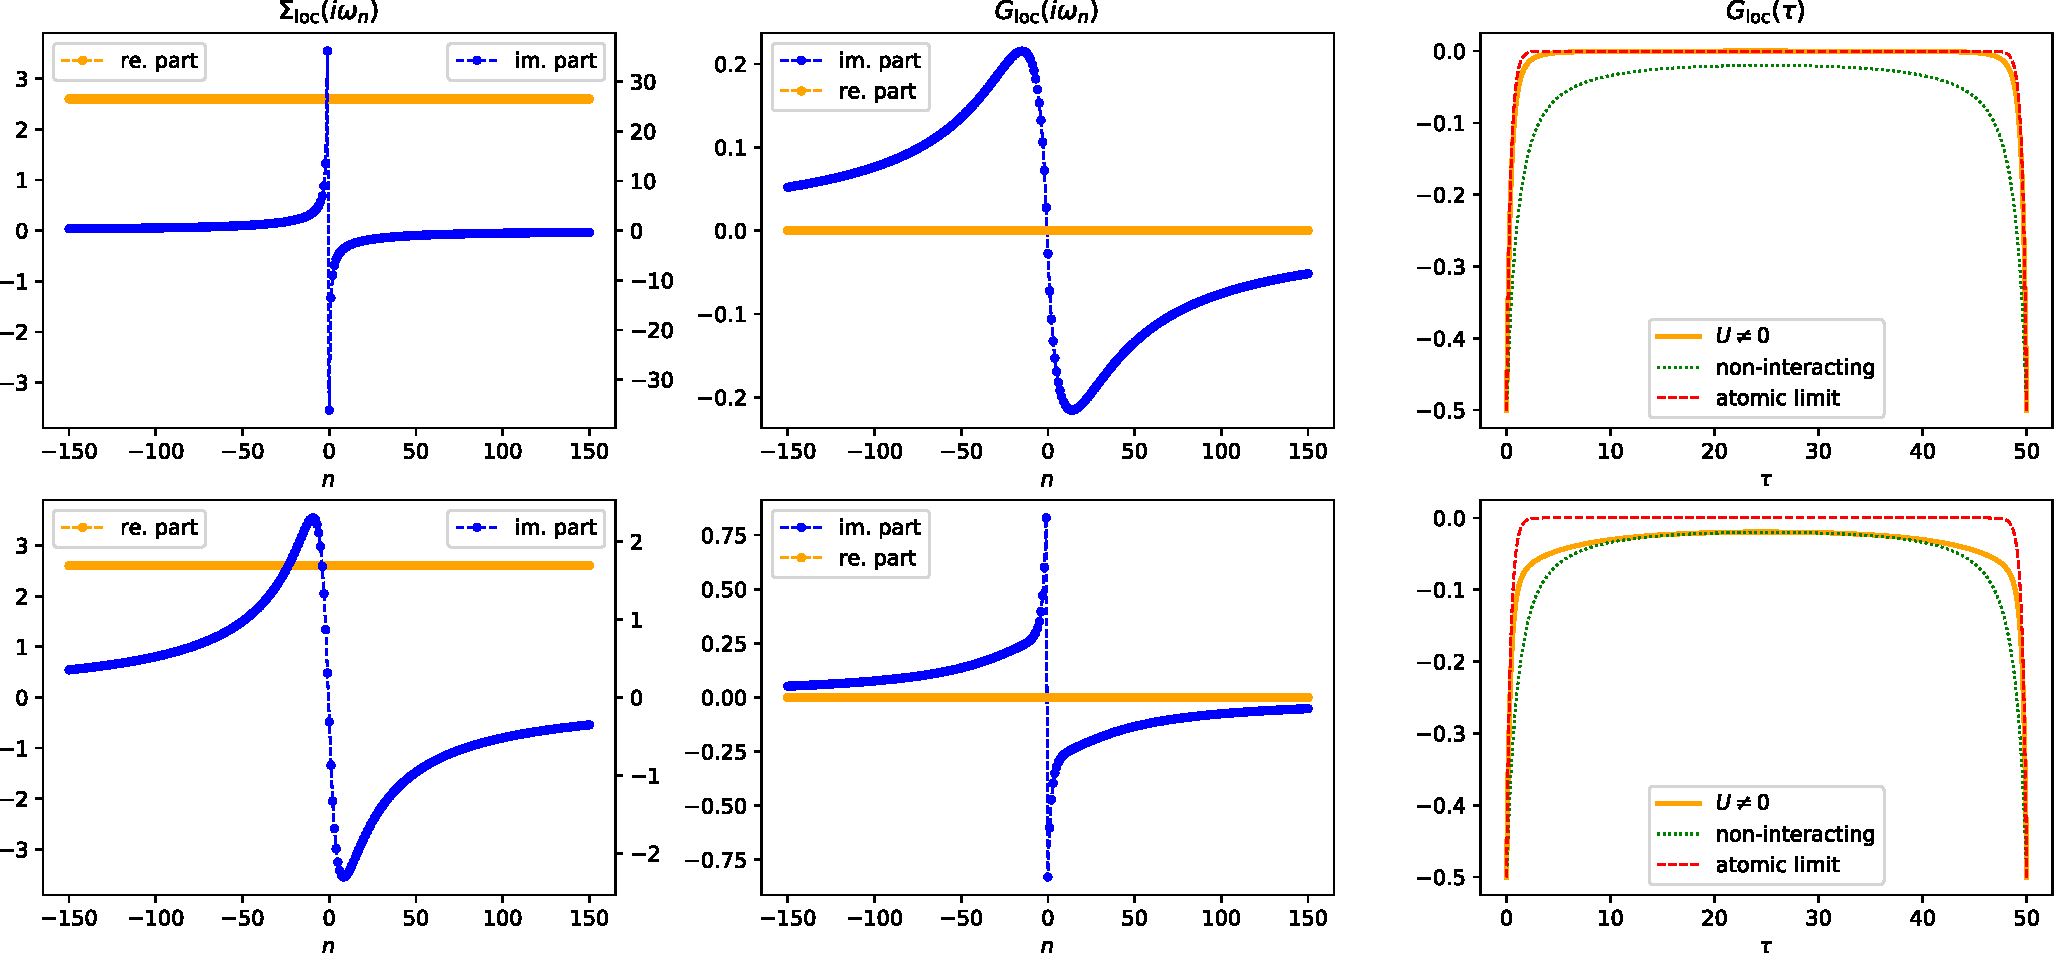
\includegraphics[width=0.92\textwidth]{U52-beta50-sigmaiwn-Giwn-Gtau-both.pdf}
\centering
\caption{\label{fig:U52-beta50-metal-insulator}Solutions to the Hubbard model on the Bethe lattice ($t=1$) in DMFT, at $U=5.2$ and $\beta=50$ ($T=0.02$). Bottom : non-interacting limit initial guess (\ref{green-func-matsubara-non-interacting}). Top : atomic limit initial guess (\ref{atomic-limit-spectral-func}). The two solutions differ, displaying meta-stability for this $(\beta,U)$. From left to right : the local self-energy, the local Green's function in Matsubara frequency space, and the local Green's function in Matsubara time space (compared to non-interacting and atomic limits). The bottom metallic self-energy shows finite zero-frequency slope, and the Green's function a $\omega=0$ pole, and thus Fermi liquid behavior (long-lifetime excitations at the Fermi surface). The top, insulating solution has no $\omega=0$ pole, and thus only has short-lifetime excitations.}
\end{figure}

\begin{figure}[H]
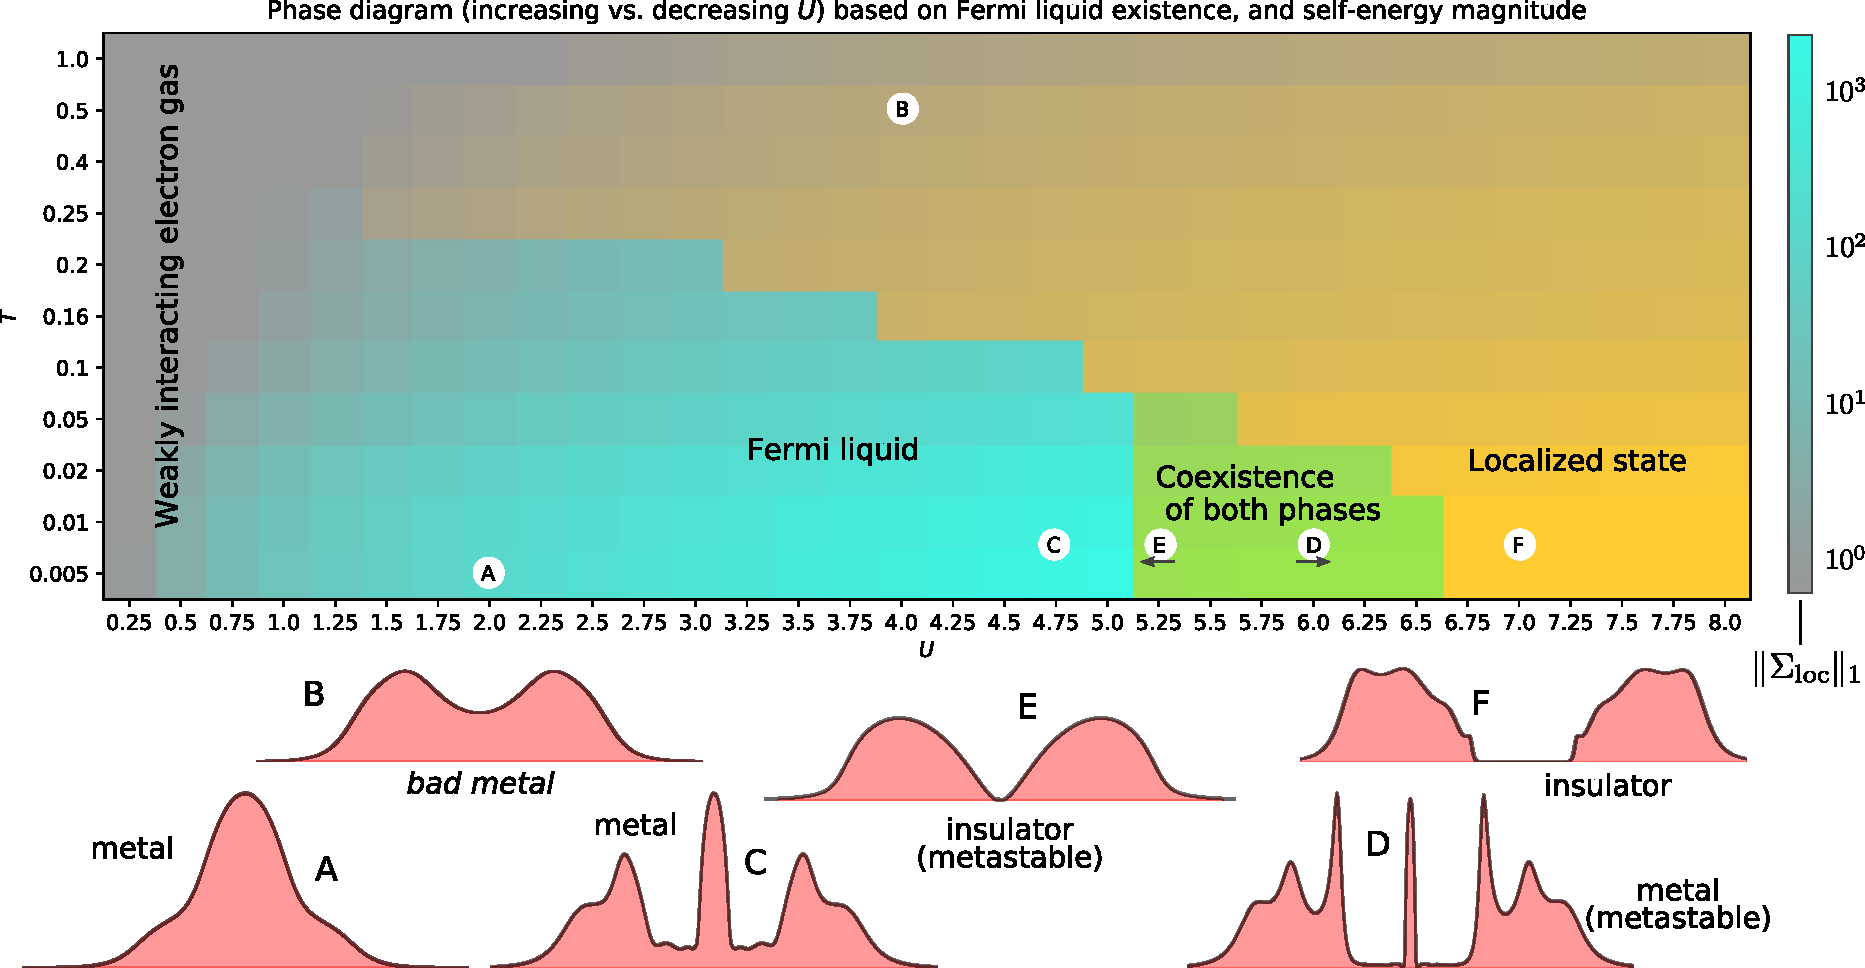
\includegraphics[width=0.925\textwidth]{phase-diagram-composition.pdf}
\centering
\caption{\label{fig:phase-diagram}The $(\beta,U)$ phase diagram of the Hubbard model on a Bethe lattice, computed by DMFT. To display meta-stability close to the transition (green area), the DMFT loop is initialized with the state of lower $U$ or larger $U$, and the two are compared. Only in the meta-stability the two resulting solutions differ.\\ The saturation of the color represents the magnitude of the self-energy $\|\Sigma(\iwn)\|_1$, which is a measure of the strength of the effects due to interactions. Grey represents negligible self-energy (the Green's function is close to the non-interacting one), while bright turquoise represents a strongly interacting Fermi liquid, and bright yellow a strongly localized state.\\Bottom : spectral functions $A(\omega)=\int\dd{\vec{k}} A(\vec{k},\omega)$ reconstructed from $G_\text{loc}$ by Padé approximants, for selected $(\beta,U)$ indicated by the respective letters. In the coexistence area, an arrow indicates if the initial guess is from increasing or decreasing $U$. Vertical scales are identical ($[0,0.32]$) and the horizontal scale is $[-6,6]$. All the diversity of states is displayed here.}
\end{figure}

\twocolumngrid

The band width of our lattice being ${\color[HTML]{008080}\epsilon} \in [-2,+2]$, the phase transition is expected (at least for low temperatures where thermal effects can be neglected) to happen around ${\color[HTML]{BF4040}U}=4$ considering eq.~\eqref{atomic-limit-spectral-func}. Actually (again, with p-h symmetry is strictly enforced in the DMFT loop), the metallic phase start to be unstable above ${\color[HTML]{BF4040}U}=5$. Fig.~\ref{fig:U52-beta50-metal-insulator} shows the resulting states at ${\color[HTML]{BF4040}U}=5.2$ and intermediate temperature. In this region, both Fermi liquid and insulating phases can exist. The displayed self-energies and Green's functions are typical, albeit very close to the critical point.

To establish a phase diagram of the Hubbard model, we run the DMFT loop for various values of $U\in[0,8]$ and $\beta\in[1,200]$. For each temperature, we vary $U$ in an increasing and in a decreasing fashion, where we use the previous $G_\text{loc}$ as the initial guess. We thus follow the hysteresis cycle, leading to phase coexistence. Where it exists, we record the quasi-particle weight \eqref{quasi-p-weight}. It is plotted on fig.~\ref{fig:quasipart-Z-incrU}.. Our main result the phase diagram in fig.~\ref{fig:phase-diagram}, established on the existence of the Fermi liquid phase.

At low temperature, the system displays the \textbf{first-order Mott transition}, which occurs between $U=5$ and $U=6.5$. To establish the exact position of the critical point $U_c$, we would have to look at other thermodynamical quantities to avoid meta-stability, as always for first order transitions. Above $U_c$, there is a \emph{gap}, so that there are no low-energy charge carriers and the system is Mott \emph{insulating} (see \raisebox{.5pt}{\textcircled{\raisebox{-.9pt} {E}}} and \raisebox{.5pt}{\textcircled{\raisebox{-.9pt} {F}}}). Below, Fermi liquid theory applies (see \raisebox{.5pt}{\textcircled{\raisebox{-.9pt} {A}}}, \raisebox{.5pt}{\textcircled{\raisebox{-.9pt} {C}}} and \raisebox{.5pt}{\textcircled{\raisebox{-.9pt} {D}}}).

Above a critical temperature $T_c\simeq 0.1$, thermal effects destroy the first order transition, and a \textbf{second-order transition} occurs. The self-energy is smaller and at high enough temperature and intermediate $U$, there is no gap anymore (see \raisebox{.5pt}{\textcircled{\raisebox{-.9pt} {B}}}) and we are in a \emph{bad metal} phase \cite{Georges_2004}.

We finally present reconstructions of $A(\omega)$ using our neural networks on fig.~\ref{fig:reconstr-final}. Only the qualitative behavior is successfully reproduced. In metallic phases, the height of the quasi-particle peak is wrong ($\neq 1/\pi$). The width of the incoherent peaks is not reproduced, but their positions (near $\pm U/2$) is. Moreover, low temperatures are much more challenging for our neural networks, which sometimes completely fail. However, the generated training dataset contains highly peaked samples which could cause the neural networks reconstructions being more peaked than the Padé ones. Modifications to the densities generation to build smoother densities could reduce this issue. Besides, the training data only containing Gaussian shapes with at most 3 peaks and not more complex shapes which can also explain the struggles of the neural networks to rebuild the final densities. However, the ability to generate as much training data as desired and the good results obtained by the networks on new data similar to the training one is promising and better data generation could lead to a broader range of reproduced densities.
\section{Conclusion}

The DMFT approach implemented with IPT successfully displays the Mott transition. The results obtained match those obtained in previous works \cite{Georges1996}. On the spectral function reconstruction with neural networks, there is plenty of room for improvements, as only a fraction of the possibilities where explored \footnote{As these networks were trained using basic CPU and GPU provided by Google, resources were somehow limited and the machine learning models were thus also designed in order to be time efficient.}.

Yet much richer physics can (and are being) explored with this tool set. The IPT limits the system to p-h symmetric states, and more versatile impurity solvers shall be used, such as Monte Carlo-based solvers or DMRG methods. We could then study itinerant ferromagnetism and establish the Stoner criterion. Even more, this model could be extended to multi-orbitals and coupled to DFT to enable us to properly study realistic materials.

However, with the tool at hands, we can already try different lattices. More time would allow us to refine the phase diagram, precisely characterize phases (such as the bad metal phases), and compute electrical and optical conductivity.

\begin{acknowledgments}
We thank Silke Biermann and Steffen Backes for taking the time to guide us through this fascinating journey. We also show appreciation to Marco Saitta for his course which gave us the interest and the opportunity to realize this project.
\end{acknowledgments}

%\vspace{10pt}
%\hrule
%\vspace{10pt}
\clearpage
\appendix
\counterwithin{figure}{section}

\section{\label{app:practical-consideration}Practical considerations}

\begin{figure}[H]
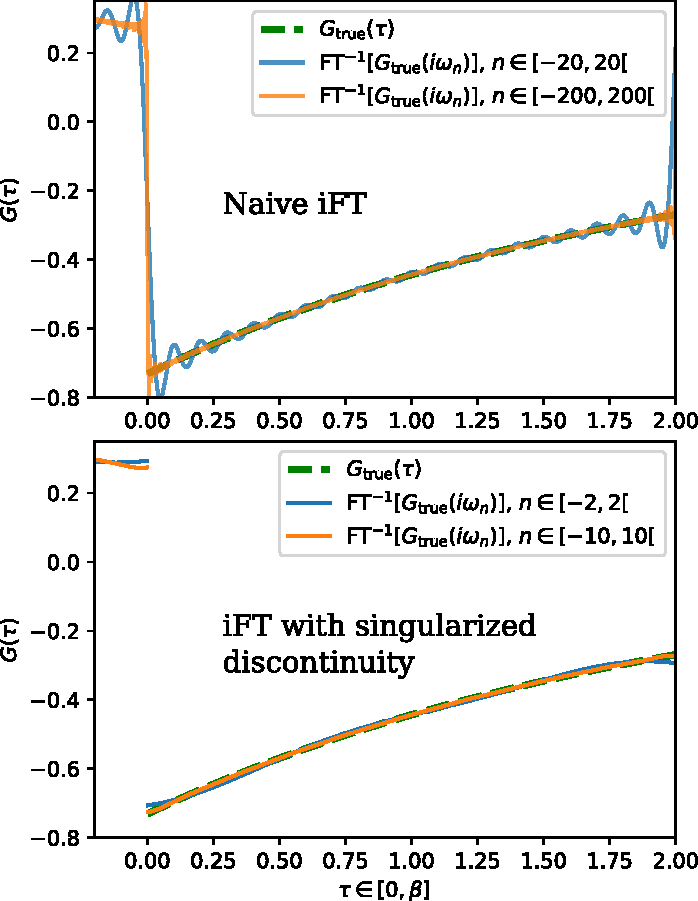
\includegraphics[width=\columnwidth]{green-tau-compar-sing.pdf}
\caption{\label{fig:green-tau-compar-sing}Green's function of the non-interacting electron gas, at $\epsilon(\vec{{k}})-\mu=0.5$. Top : exact Green function, and iFT of the exact $G(\iwn)$. Even with high frequency cutoffs, Gibbs ringing is unacceptable. Bottom : iFT computed with eq.\ \ref{iFT-sing}. There is no ringing anymore, and even very small cutoffs ($n_\text{cut}=10$) approximate well the true function.}
\end{figure}

\begin{figure*}
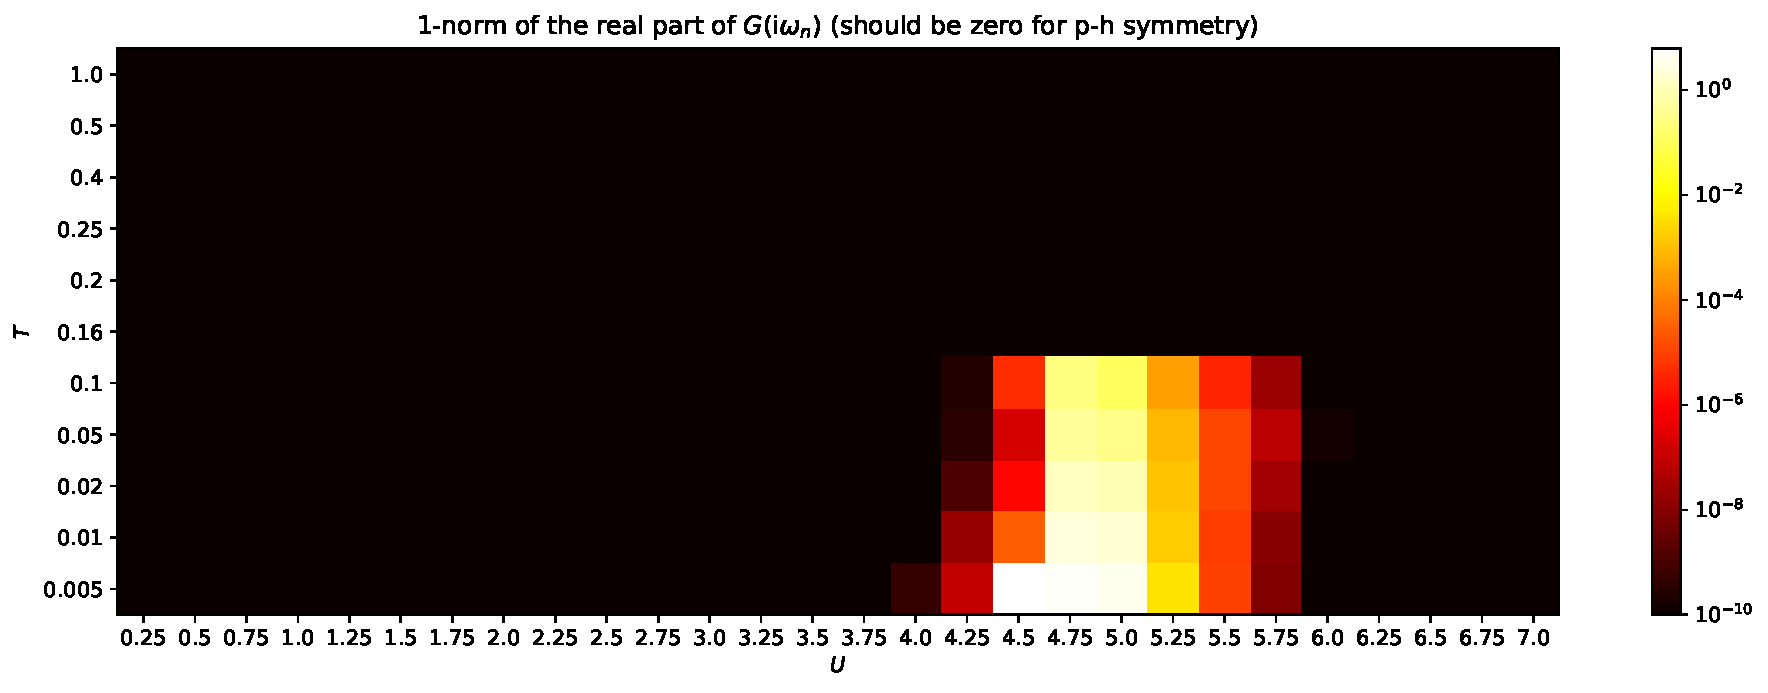
\includegraphics[width=\textwidth]{real-part-norm-increasingU.pdf}
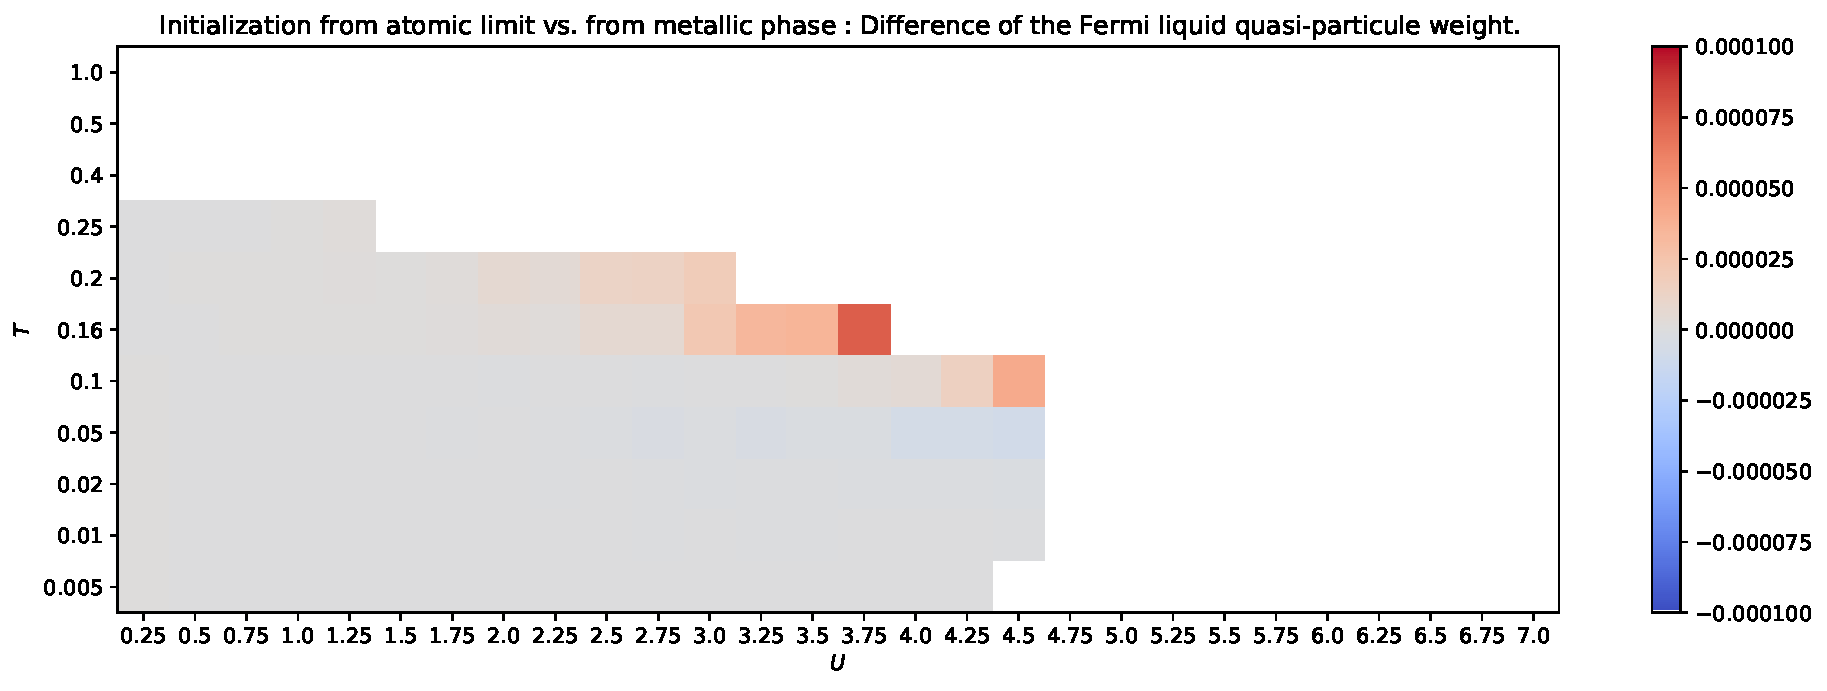
\includegraphics[width=\textwidth]{diff-Zat-ZincU.pdf}
\caption{\label{fig:ph-diag-sanity-checks}Top : unwanted real part of $G_\text{loc}(\iwn)$ when no p-h symmetry is imposed. There is symmetry breaking near the transition. We can't trust the IPT in such cases. Bottom : difference of the quasi-particle weight $\mathcal{Z}$ (where it is defined) in the phase space $(\beta, U)$, between two runs of the DMFT loop (worse case) : initialization from atomic limit state vs.\ metallic state.}
\end{figure*}

\section{Neural networks parameter optimization}

\subsection{Gradient descent\label{sec:nn:grad-desc}}

\begin{itemize}
    \item Adam optimizer is used (with Keras default parameters) as it yields more accurate results than stochastic gradient descent or RMSprop optimisers for instance. This is explained by the fact that it wasn't suffering from the gradient vanishing problems the other optimisers were facing which damaged their ability to keep learning over time.
    \item A batch size of 128 was chosen to get a meaningful approximation of the gradient but still perform many updates of the parameters for each epoch.
\end{itemize}

\subsection{Choice of the norm\label{sec:nn:norm}}

\begin{figure}[H]
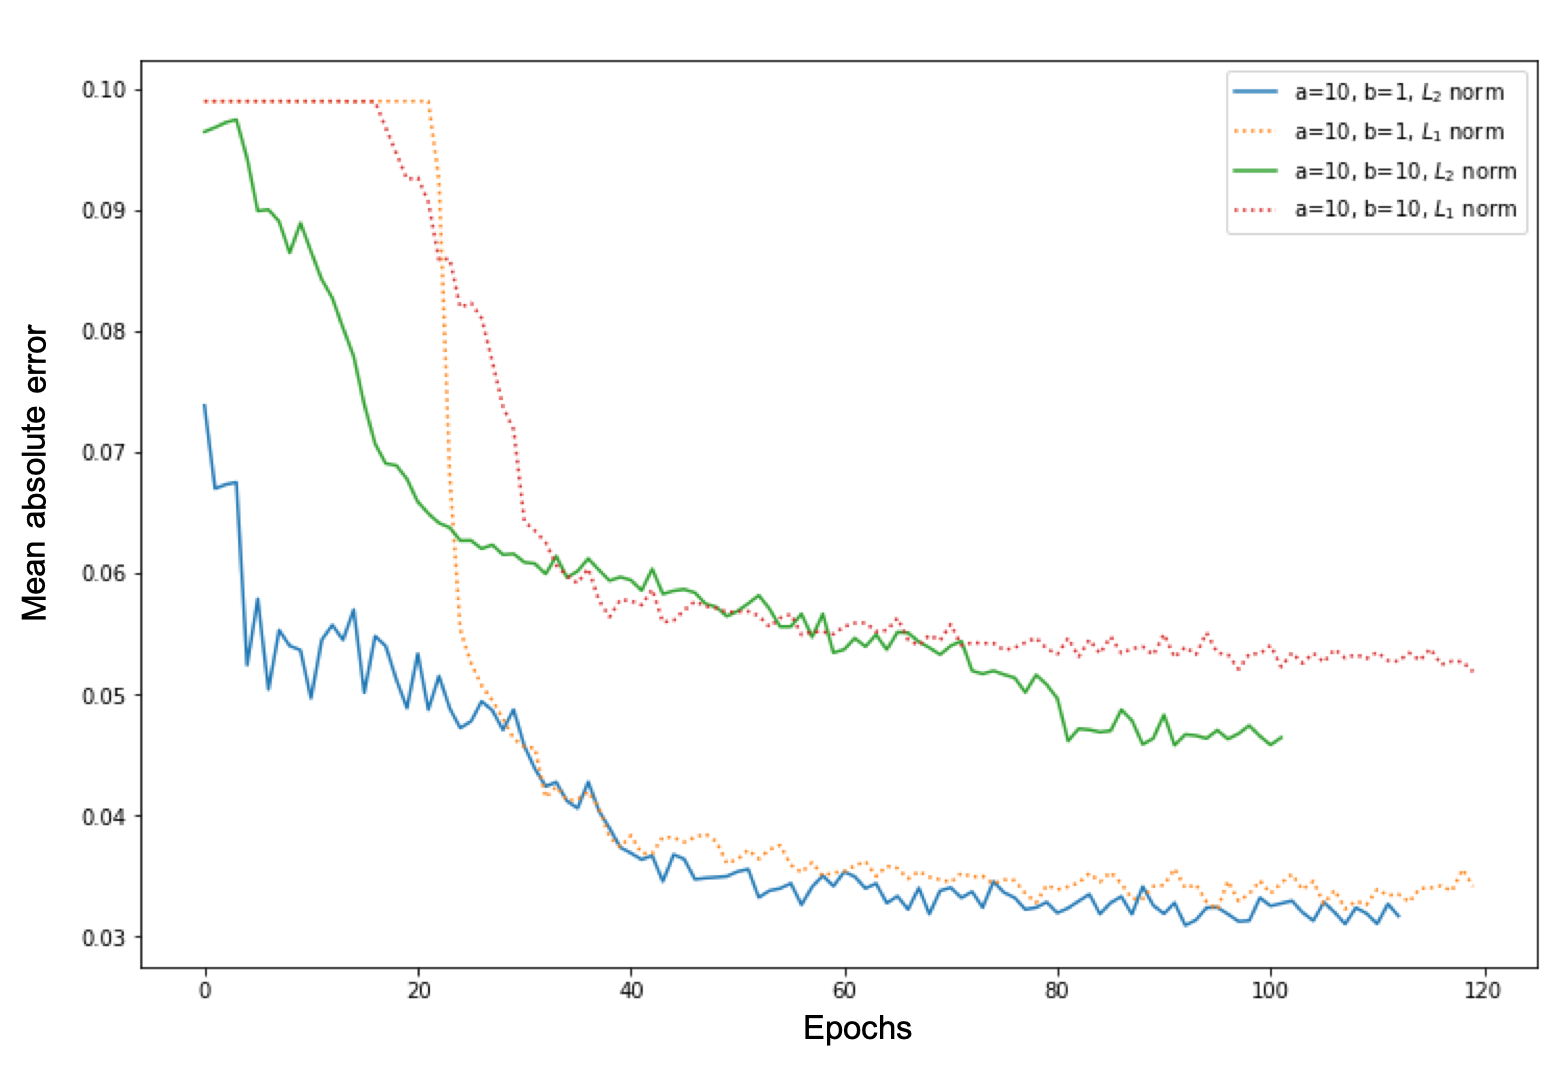
\includegraphics[width=\columnwidth]{analytical_continuation/norm_weighting_final.png}
\caption{\label{fig:norm1_or_2}Evolution of the validation MAE over time with different norms and weighting.}
\end{figure}

As a few examples illustrate it on Figure~\ref{fig:norm1_or_2}, the use of $L_1$ seemed to create a surprising "plateau" behavior and the beginning of training and yields a bit less accurate results. 

\section{Additional results}

The Fermi liquid quasi-particle weight is plotted in the phase space on fig.~\ref{fig:quasipart-Z-incrU}.

\begin{figure*}
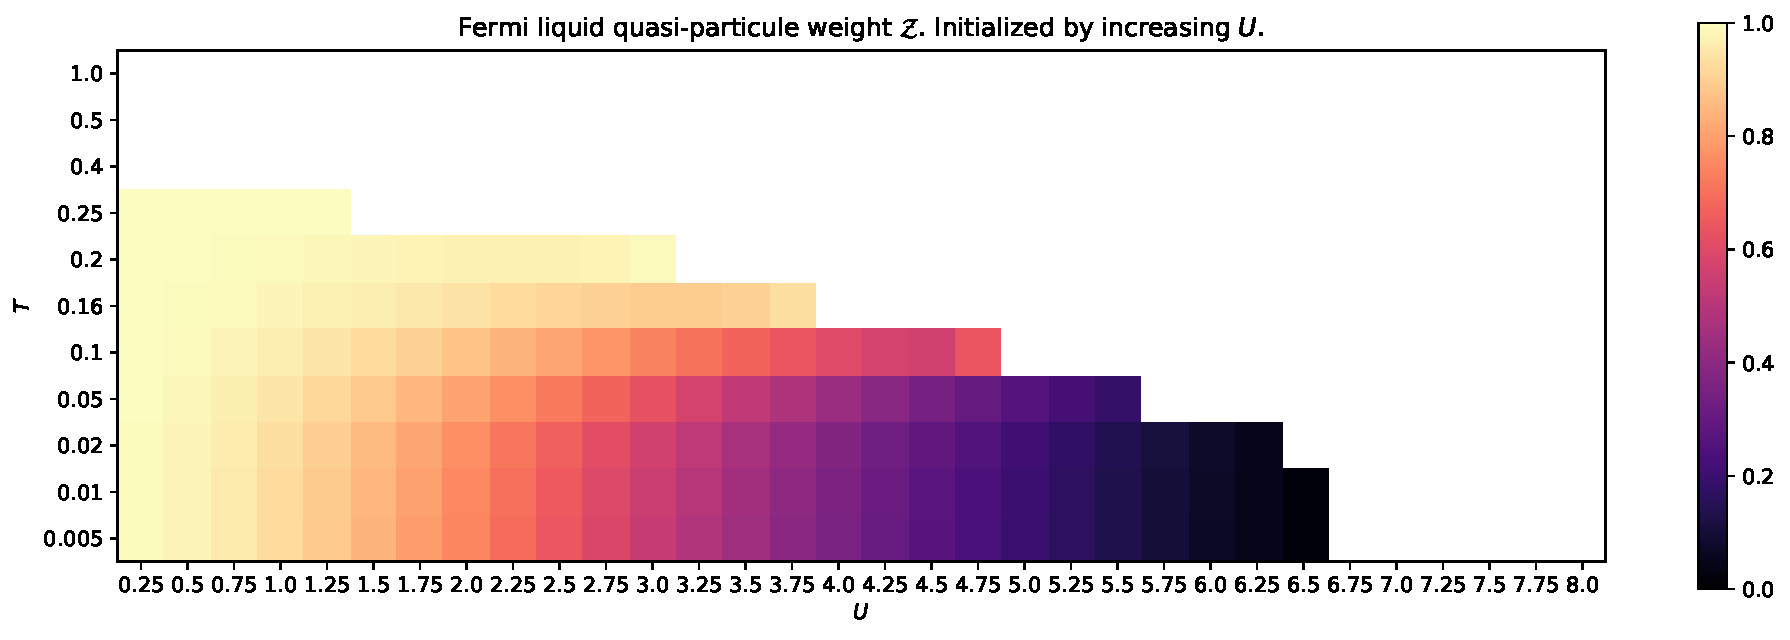
\includegraphics[width=\textwidth]{quasipart-Z-incrU.pdf}
\caption{\label{fig:quasipart-Z-incrU}Value of the quasi-particle weigh $\mathcal{Z}$ computed from $\Sigma_\text{loc}$ in the $(\beta,U)$ space, and with increasing $U$ (Fermi liquid side of the hysteresis cycle).}
\end{figure*}

\section{Anderson impurity model}\label{impurity_model_section}

The \textit{Anderson impurity model} is a many-body fermionic model describing a single site, with repulsive Coulomb interaction, coupled to a bath allowing for charge fluctuations. With discretized bath levels $\ell$ (as illustrated on fig~\ref{fig:sch-impurity-mapping}), its hamiltonian reads
\begin{equation}
  \tmbf{H}_{\text{imp}}^{\mathrm{{\tmname{gc}}}} =
  {\color[HTML]{800080}\tmbf{H}_{\text{site}}} +
  {\color[HTML]{000080}\tmbf{H}_{\text{coupl}}} +
  {\color[HTML]{000080}\tmbf{H}_{\text{bath}}}
\label{impurity-hamiltonian}
\end{equation}
\centerline{where}
\[
  \left\{\begin{array}{l}
    {\color[HTML]{800080}\tmbf{H}_{\text{site}}} =  - \mu
    ({\color[HTML]{800080}\tmbf{n}}_{\uparrow} +
    {\color[HTML]{800080}\tmbf{n}}_{\downarrow}) + {\color[HTML]{BF4040}U}
    {\color[HTML]{800080}\tmbf{n}}_{\uparrow} 
    {\color[HTML]{800080}\tmbf{n}}_{\downarrow} \quad (\tmbf{n}=
    {\color[HTML]{800080}\tmbf{c}}^{\dag} 
    {\color[HTML]{800080}\tmbf{c}})\\
    {\color[HTML]{000080}\tmbf{H}_{\text{bath}}} = \sum_{\ell \sigma}
    {\color[HTML]{000080}E_{\ell}}  {\color[HTML]{000080}\tmbf{a}}_{\ell
    \sigma}^{\dag}  {\color[HTML]{000080}\tmbf{a}}_{\ell \sigma}\\
    {\color[HTML]{000080}\tmbf{H}_{\text{coupl}}} = \sum_{\ell \sigma}
    {\color[HTML]{000080}V_{\ell}}  ({\color[HTML]{000080}\tmbf{a}}_{\ell
    \sigma}^{\dag}  {\color[HTML]{800080}\tmbf{c}}_{\sigma} +
    {\color[HTML]{800080}\tmbf{c}}_{\sigma}^{\dag} 
    {\color[HTML]{000080}\tmbf{a}}_{\ell \sigma})
  \end{array}\right.  
\]

The natural framework for relating the initial Hubbard model and the impurity
model is the one of Green's functions. In the initial problem, the Green's
function describes processes on-site $\vec{R} \rightarrow \vec{R}$
(${\color[HTML]{BF4040}G}_{i i} \equiv {\color[HTML]{BF4040}G}_{\text{loc}}$,
the {\tmem{local part of the Green's function}}) but also {\tmem{between}}
sites $\vec{R}_i \rightarrow \vec{R}_j$ (${\color[HTML]{BF4040}G}_{i j}$). However, in the impurity model,
there is only the impurity Green's function \eqref{Gimp-def}, which we require to be identical to ${\color[HTML]{BF4040}G}_{\text{loc}}^\text{latt}$. This is the LISA.

The {\color[HTML]{000080}bath} $\{ {\color[HTML]{000080}\tmbf{a}}_{\ell
\sigma}^{\dag} \}$ is described by effective energy levels
${\color[HTML]{000080}\epsilon_{\ell}}$. The effective coupling constants ${\color[HTML]{000080}V_{\ell}}$ and effective energy levels
${\color[HTML]{000080}\epsilon_{\ell}}$ {\tmem{are chosen/solved so as to reproduce our initial Hubbard system self-consistently}} at a given
${\color[HTML]{BF4040}U}$. However, there is an unnecessary freedom of choice
and complexity in this description and we'd better of using an action representation of $\tmbf{H}_{\text{imp}}^{\mathrm{{\tmname{gc}}}}$ :
\begin{eqnarray*}
  \tmbf{S}^\text{imp} &=& {- \int_0^{\beta} \dd{\tau}
  \int_0^{\beta} \dd{\tau'}}  {\color[HTML]{800080}\tmbf{c}}^{\dag}
  (\tau)  \frac{1}{{\color[HTML]{000080}\mathcal{G}_0} (\tau - \tau')} 
  {\color[HTML]{800080}\tmbf{c}}(\tau)\\ &&\ + {\color[HTML]{BF4040}U}  \int_0^{\beta} \dd{\tau} {\color[HTML]{800080}\tmbf{n}}_{\uparrow} (\tau) {\color[HTML]{800080}\tmbf{n}}_{\downarrow}(\tau)
  \label{impurity-action}
\end{eqnarray*}
where the degrees of freedom of the bath has been formally
integrated into the \emph{bath Green's
function} ${\color[HTML]{000080}\mathcal{G}_0}$ :
\begin{equation*}
  {\color[HTML]{000080}\mathcal{G}_0} (\iwn) = \frac{1}{\mathi
  \omega_n + \mu - {\color[HTML]{000080}\Delta} (\mathi
  \omega_n)},\ {\color[HTML]{000080}\Delta} (\mathi
  \omega_n) = \sum_{\ell} \frac{| {\color[HTML]{000080}V_{\ell}} |^2}{\mathi
  \omega_n - {\color[HTML]{000080}E_{\ell}}} \label{bath-G-with-Delta-func}
\end{equation*}

We have to compute this mean field ${\color[HTML]{000080}\mathcal{G}_0}$ acting on the impurity. This is done through the cavity method \cite{Georges1996}, which establishes the expression of the bath as function of the lattice and its $t_{ij}$'s : ${\color[HTML]{000080}\Delta} = {\color[HTML]{BF4040}\zeta} - 1/{{\color[HTML]{008080}\tilde{\eta}}
({\color[HTML]{BF4040}\zeta})}$ where ${\color[HTML]{BF4040}\zeta} (\mathi
\omega_n) = \iwn + \mu -{\color[HTML]{BF4040}\Sigma}_{\text{loc}} (\iwn)$ and where ${\color[HTML]{008080}\tilde{\eta}}$ is the Hilbert transform of the density of states, giving us
\begin{equation} {\color[HTML]{000080}\mathcal{G}_0} (\iwn)^{- 1} = 
   {\color[HTML]{BF4040}\Sigma}_{\text{loc}} (\iwn) +
   \frac{1}{{\color[HTML]{008080}\tilde{\eta}} ({\color[HTML]{BF4040}\zeta}
   (\iwn))} \end{equation}
It is expressed synthetically as a function of ${\color[HTML]{BF4040}G}_{\text{loc}} = {\color[HTML]{008080}\tilde{\eta}} ({\color[HTML]{BF4040}\zeta})$:
\begin{equation} {\color[HTML]{BF4040}\Sigma}_{\text{loc}} =
   \frac{1}{{\color[HTML]{000080}\mathcal{G}_0}} -
   \frac{1}{{\color[HTML]{BF4040}G}_{\text{loc}}} \end{equation}
A third expression can be obtained if we consider ${\color[HTML]{008080}R}$, the reciprocal function of ${\color[HTML]{008080}\tilde{\eta}} (\zeta)$ :
\begin{equation}
    {\color[HTML]{000080}\mathcal{G}_0} (\iwn)^{- 1} = \iwn + \mu + {\color[HTML]{BF4040}G}_{\text{loc}} (\iwn)^{- 1} - {\color[HTML]{008080}R} ( {\color[HTML]{BF4040}G}_{\text{loc}} (\iwn) )
    \label{self-consistent-eq-reciproc-Hilbert}
\end{equation}

\bibliography{main}

\end{document}